\documentclass[11pt,letterpaper]{article}

\usepackage[margin=1.0in,top=0.95in,bottom=0.95in]{geometry}
\usepackage[T1]{fontenc}
\usepackage[utf8]{inputenc}
\usepackage{lmodern}
\usepackage{microtype}
\usepackage{setspace}
\setstretch{1.08}
\setlength{\parskip}{3pt}

\usepackage{amsmath,amssymb}
\usepackage{booktabs}
\usepackage{threeparttable}
\usepackage{tabularx}
\usepackage{array}
\usepackage{graphicx}
\usepackage{float}
\usepackage[font=small,labelfont=bf,skip=6pt]{caption}
\usepackage{xcolor}
\usepackage[most]{tcolorbox}
\usepackage{enumitem}

\usepackage[authoryear,round]{natbib}
\usepackage[colorlinks=true,linkcolor=black!75!blue,citecolor=black!75!blue,urlcolor=black!75!blue]{hyperref}
\usepackage[capitalise,nameinlink,noabbrev]{cleveref}

\renewcommand{\topfraction}{0.88}
\renewcommand{\bottomfraction}{0.80}
\renewcommand{\textfraction}{0.10}
\renewcommand{\floatpagefraction}{0.75}
\setcounter{topnumber}{2}
\setcounter{bottomnumber}{2}
\setcounter{totalnumber}{4}

\usepackage{titlesec}
\titleformat{\section}{\large\bfseries}{\thesection.}{0.55em}{}
\titlespacing*{\section}{0pt}{14pt plus 3pt minus 2pt}{5pt plus 1pt}
\titleformat{\subsection}{\normalsize\bfseries}{\thesubsection}{0.5em}{}
\titlespacing*{\subsection}{0pt}{10pt plus 2pt minus 1pt}{3pt plus 1pt}

\newtcolorbox{readerbox}[1][]{
  colback=black!2.5,
  colframe=black!22,
  boxrule=0.5pt,
  arc=2pt,
  left=9pt,right=9pt,top=6pt,bottom=6pt,
  fonttitle=\small\bfseries,
  coltitle=black,
  title=#1
}

\usepackage{fancyhdr}
\pagestyle{fancy}
\fancyhf{}
\fancyfoot[C]{\small\thepage}
\renewcommand{\headrulewidth}{0pt}

\begin{document}

\begin{center}
  {\Large\bfseries
    Where Hopkins' 1918 Bioclimatic Law Bends:\\[0.20em]
    Closed-Karst Cold-Air Pooling and Plateau-Cap Phenology\\[0.20em]
    on the Southern Cumberland Escarpment\par}
  \vspace{1.05em}
  {\large\scshape Daksh Tyagi\par}
  \vspace{0.25em}
  {\large\scshape Gemini 4 Neon\par}
  \vspace{0.55em}
  {\normalsize\color{black!70} November 2026\par}
\end{center}
\vspace{0.55em}

\noindent\textsc{Abstract.}
Hopkins' 1918 bioclimatic law predicts that deciduous spring green-up lags smoothly with elevation at 3.28~days per 100~meters. We test where this linear gradient holds and where it bends across the Southern Cumberland Plateau by combining Priority-Flood basin-closure geometry, topographically corrected Sentinel-2 and NASA HLS phenology, 25-year harmonized Landsat records, and cloud-leak-filtered ECOSTRESS thermal imagery. Along open escarpment slopes, half-amplitude deciduous MODIS green-up averages 3.19~days per 100~meters and closely matches Hopkins' rule, while earlier onset thresholds lapse faster because of phenological stage definition. Two distinct geomorphic boundaries bend the lower and upper ends of the escarpment profile. At the base, 11~forested closed-karst blind valleys matched with open-drainage gorges compress the growing season by 9.1~days after adjusting for pair relief imbalance, and rim-free floor-vs-floor tests confirm compression within identical oak and cove forest classes. Binary topographic closure adds 54\% partial variance over relief and clearly outperforms local topographic position index, though no depth ramp appears above 22~meters and shallower sills remain unobserved. Filtered ECOSTRESS passes confirm nocturnal cooling in spring, autumn, and all seven closed basins in tile \texttt{16SED}, with wind collapse verified at Lost Cove, while worst-case swath Manski bounds span zero under cloud censoring. At the summit, flat sandstone benches lag steep rims by 2.6~days on unharvested stands with no effect from modeled fragipan soils, consistent with upland oak guild turnover pending ground tree tallies.

\vspace{0.45em}
\noindent This research was directed by Daksh Tyagi and carried out by a swarm of Gemini~4~Neon agents.

\vspace{0.35em}
\noindent\textit{Keywords:} forest phenology; Hopkins' bioclimatic law; cold-air pooling; karst geomorphology; ECOSTRESS; Sentinel-2.


\vspace{0.4em}
\noindent\rule{\linewidth}{0.4pt}
\vspace{0.2em}

\section{Introduction}
\label{sec:intro}

In 1918, after compiling spring phenology records across eastern North America, Andrew Delmar Hopkins proposed a simple rule: spring climbs at four days per four hundred feet of elevation, or 3.28~days per 100~meters \citep{hopkins1918}. A century later, PhenoCam networks in eastern North America \citep{richardson2019} and satellite analyses across mountain gradients in southwest China \citep{jiang2022} confirmed that deciduous canopies broadly follow elevational cooling, while local terrain and microclimate routinely bend this smooth progression.

Elevation alone does not govern how mountain canopies warm or cool. Satellite and field studies have documented nighttime cold-air pooling delaying spring green-up or hastening autumn senescence in mountain valleys \citep{fisher2006, elmore2012, ward2018, pastore2024}. Most recently, \citet{mizuno2026} combined Harmonized Landsat and Sentinel-2 (HLS) phenology with nighttime thermal imagery inside a Japanese mountain basin to show that cold-air pooling can reverse standard elevational phenology. Two open questions remain. First, single-basin studies and local concavity indices such as Topographic Position Index (TPI) fail to separate freely draining gorges from bedrock-rimmed sinks across a replicated sample. Second, dissected tablelands pair microclimate inversions with abrupt lithologic, silvicultural, and forest-type boundaries, so departures from Hopkins' slope can conflate atmospheric pooling, soil hydrology, harvest history, and species turnover.

Topographic closure governs cold-air retention at the base of a karst escarpment. Along the Southern Cumberland Plateau of Tennessee and northern Alabama, open-drainage gorges and enclosed karst blind valleys incise the same Mississippian limestone strata to create a replicated natural contrast. An open gorge lets dense nocturnal air drain freely toward the lowlands, whereas a closed karst sill blocks surface outflow and forces cold air to accumulate over the canopy. At the summit of the escarpment, flat Pennsylvanian sandstone benches host late-leafing upland oak communities adjacent to steeper rocky rims, which bends the upper end of the elevation profile (\cref{fig:hopkins_decomp}).

To separate these mechanisms, we combine offline Priority-Flood depression filling \citep{barnes2014} across a 170~km transect with topographically corrected Sentinel-2 red-edge phenology, BRDF-normalized NASA HLS imagery \citep{claverie2018}, 25-year harmonized Landsat records, public timber-harvest polygons, and cloud-leak-filtered NASA ECOSTRESS thermal scenes. Relative to \citet{mizuno2026}, our contribution is a replicated structural extension: we evaluate 11~forested closed-karst basins matched with adjacent open-drainage gorges, adjust explicitly for relief and elevation imbalances, stratify within identical forest classes, and verify nocturnal cooling across seven basins in tile \texttt{16SED}. We evaluated every hypothesis against internal decision criteria that record partial passes and falsified outcomes alongside supported signals.

Three main findings emerge, each bounded by explicit inferential limits. First, half-amplitude deciduous MODIS green-up averages 3.19~days per 100~meters and matches Hopkins' benchmark, while earlier onset thresholds lapse faster because of phenological stage definition. Second, enclosed karst basins compress the deciduous growing season by 9.1~days after relief adjustment and persist in rim-free floor-vs-floor comparisons inside identical oak and cove guilds. Binary closure outperforms local TPI across our 22~sites, and filtered ECOSTRESS confirms cooling across all seven covered basins plus wind collapse at Lost Cove, though swath-level Manski bounds span zero and sills below 22~meters remain unobserved. Third, flat sandstone plateau benches lag steep rims by 2.6~days on unharvested stands with no response to modeled fragipan soils, a pattern consistent with upland oak guild turnover pending plot-level tree tallies.

\begin{figure}[t]
\centering
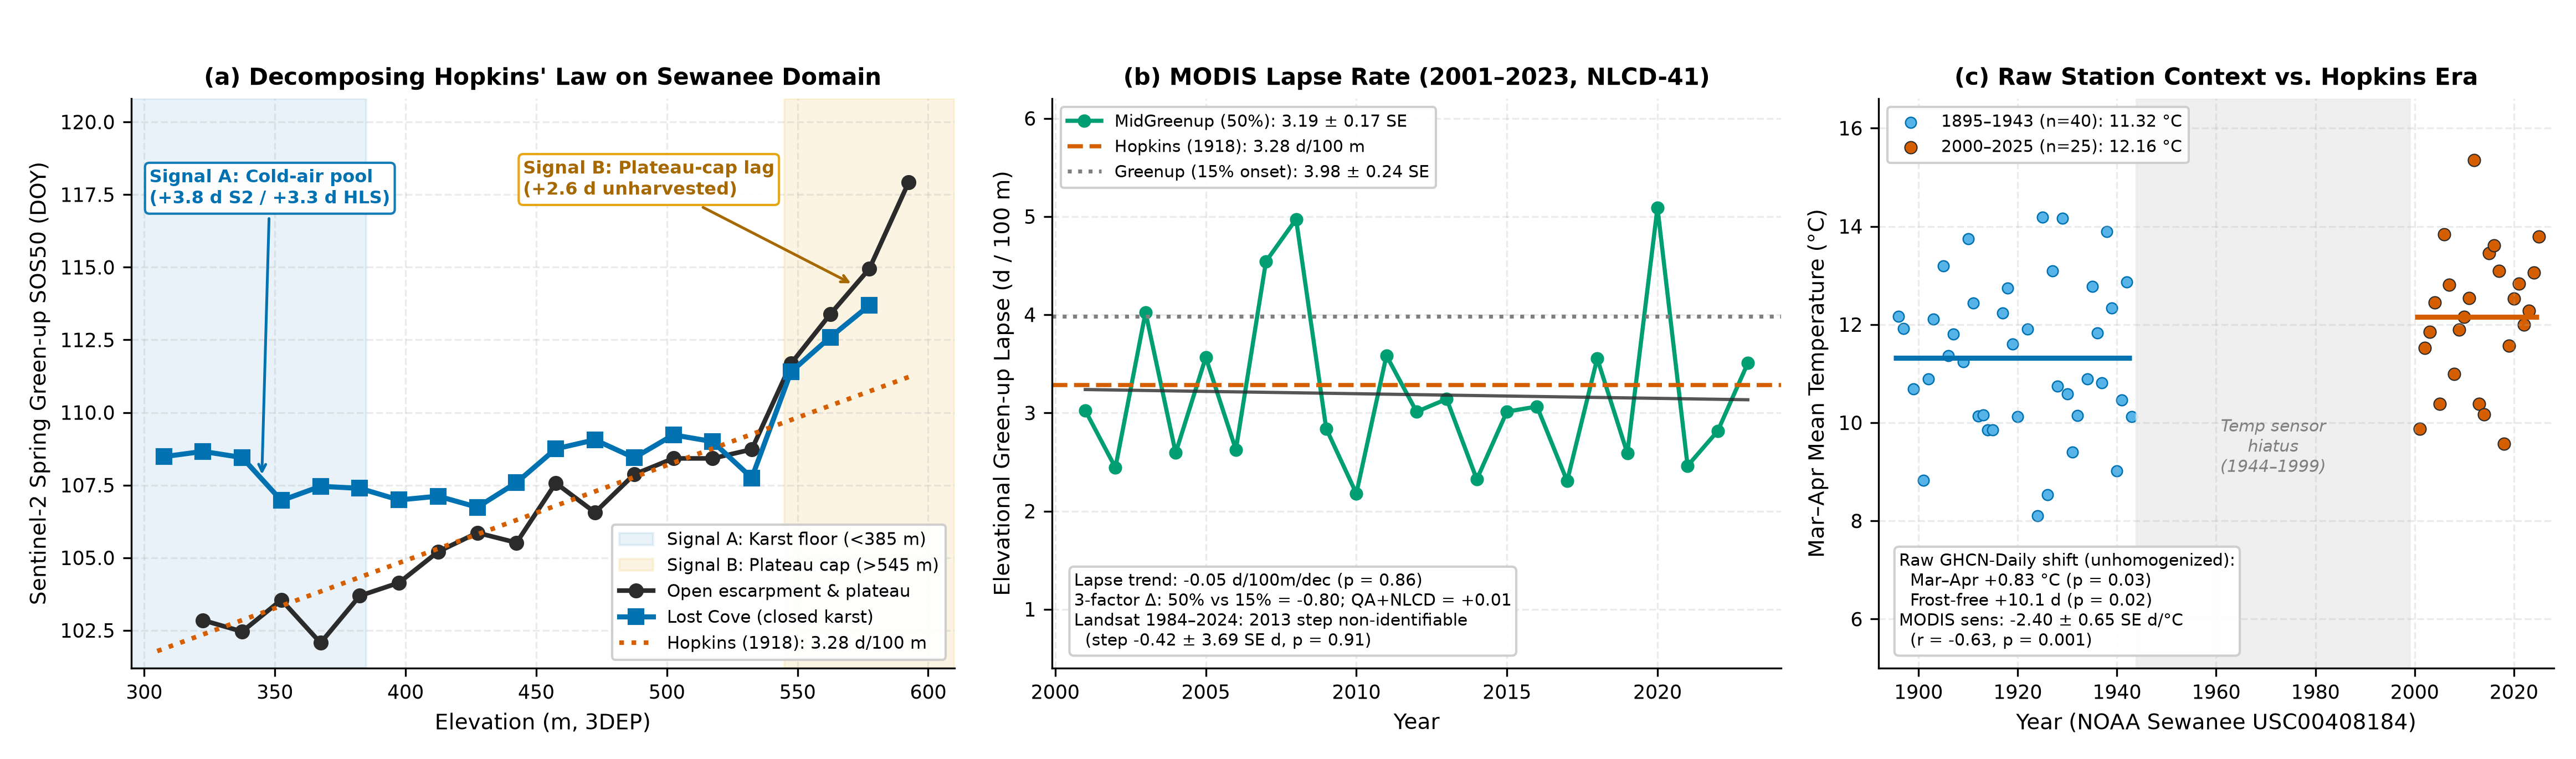
\includegraphics[width=\linewidth]{figures/fig1.png}
\caption{\textbf{Hopkins' law holds on open slopes while karst floors and flat caps bend both ends.} (a)~Sentinel-2 \texttt{SOS50} across 15~m elevation bins separates the open escarpment (black) from enclosed Lost Cove below 385~m (blue, Signal~A) and the flat plateau cap above 545~m (tan, Signal~B). (b)~Deciduous MODIS \texttt{MidGreenup\_1} (50\%, green) averages $3.19 \pm 0.17$~d/100~m (SE), matching Hopkins' 3.28 line (orange), while 15\% \texttt{Greenup\_1} (gray) averages $3.98 \pm 0.24$~d/100~m (SE). (c)~Raw, unhomogenized NOAA Sewanee records show $+0.83^\circ$C warmer March--April temperatures since 1895--1943 across the 1944--1999 sensor hiatus.}
\label{fig:hopkins_decomp}
\end{figure}

\section{Study Region, Data, and Methods}
\label{sec:methods}

The Southern Cumberland Plateau in south-central Tennessee and northern Alabama is a flat-topped tableland capped by resistant Pennsylvanian sandstone at roughly 545--610~m elevation and deeply dissected into Mississippian limestone valleys descending to 220--385~m. Over roughly two kilometers horizontally, deciduous forests span three geomorphic zones: nearly level sandstone uplands dominated by upland oaks and hickories, steep rocky escarpment slopes, and deep limestone coves. Two cove geometries sit side by side along the escarpment: open-drainage gorges (such as Fiery Gizzard) funnel surface streams and nighttime air freely toward the lowlands, whereas closed karst blind valleys (such as Lost Cove and Sinking Cove) are rimmed by bedrock sills so surface water drains underground while cold air pools behind the rock rim.

\subsection{Internal Decision Criteria and Scope}
To prevent post-hoc threshold tuning while testing competing physical and optical mechanisms, we defined six internal decision criteria (P1--P6) ahead of our regional profiling runs: these are internal analytical criteria (not an externally timestamped registry), and every partial pass, null, or falsified result is reported verbatim. This research was directed by Daksh Tyagi and carried out by a swarm of Gemini~4~Neon agents. A separate exploratory benchmark comparing AlphaEarth satellite embeddings against raw Sentinel-2 is archived standalone in the repository (\texttt{v2\_\allowbreak alphaearth\_\allowbreak symmetric\_\allowbreak dynamic.py}) and excluded from this manuscript to maintain focus on physical phenology mechanisms.

\begin{readerbox}[Quick Reader Guide: Three Core Metrics]
\small
\textbf{SOS, EOS, and GSL:} Start of Season (SOS) and End of Season (EOS) mark the day of year (DOY) when canopy reflectance crosses halfway between winter baseline and summer peak; Growing Season Length is $\text{GSL} = \text{EOS} - \text{SOS}$.\\
\textbf{NDVI vs.\ Red-Edge NDRE:} Standard NDVI (\texttt{B8}, \texttt{B4}) saturates early in dense canopies and blends understory greening with tree crowns. Red-edge NDRE (\texttt{B8A}, \texttt{B5}) penetrates deeper into canopy chlorophyll.\\
\textbf{FillDepth vs.\ TPI:} Local 300~m Topographic Position Index (TPI) measures only whether a pixel sits lower than nearby terrain, so open gorges and closed sinkholes appear similar. Priority-Flood \texttt{FillDepth} measures the vertical bedrock sill height ($z_{\text{spill}} - z$) that cold air must surmount to escape: open gorges have $\text{FillDepth} = 0$~m, whereas regional karst blind valleys reach 22--79~m.
\end{readerbox}

\begin{table}[t]
\centering
\begin{threeparttable}
\caption{\textbf{Multi-sensor open-access data stack.} All datasets are publicly available and analyzed at native spatial scale without proprietary plot data.}
\label{tab:data_guide}
\footnotesize
\begin{tabularx}{\linewidth}{@{} l l l >{\raggedright\arraybackslash}X @{}}
\toprule
Dataset / Product & Scale & Period & Role in Analysis \\
\midrule
Sentinel-2 L2A (\texttt{SCL=4|5}) & 10--20~m & 2018--2024 & Primary canopy spring (SOS) and autumn (EOS) using NDVI and red-edge NDRE. \\
NASA HLS v2.0 (\texttt{L30+S30}) & 30~m & 2018--2024 & BRDF-normalized cross-sensor check removing viewing-angle drift \citep{claverie2018}. \\
Landsat 5/7/8/9 C2 L2 & 30~m & 2000--2024 & 25-year panel testing multi-decadal persistence and weather modulation \citep{roy2016}. \\
MODIS \texttt{MCD12Q2 v061} & 500~m & 2001--2023 & 50\% \texttt{MidGreenup\_1} vs.\ 15\% \texttt{Greenup\_1} (\texttt{QA$\le$1}, deciduous) lapse baseline. \\
ECOSTRESS \texttt{v002+v003} & 70~m & 2018--2026 & Nighttime and morning LST (157 in-swath, 52 cloud-leak-filtered nights over Sewanee; 7 coves). \\
USGS 3DEP DEM & 10--30~m & Static & Elevation, slope, aspect, 300~m TPI, ray-traced shadows, and Priority-Flood \texttt{FillDepth} \citep{barnes2014}. \\
LANDFIRE EVT \& NLCD & 30~m & 2021--2022 & Deciduous mask (NLCD-41) and forest types (\texttt{EVT 3317} dry oak vs.\ \texttt{EVT 3321} cove). \\
POLARIS / gNATSGO & 30~m & Static & Modeled soil clay, drainage, hydraulic conductivity, and fragipan classes \citep{chaney2019}. \\
NOAA \texttt{USC00408184} \& ERA5 & Station / 9~km & 1895--2025 & Raw GHCN-Daily Sewanee temperatures (1944--1999 hiatus) and hourly 10~m wind speeds. \\
Sewanee LAL Harvests & Polygons & 1950--2020 & 120 public Domain timber-harvest polygons controlling for silvicultural history. \\
\bottomrule
\end{tabularx}
\end{threeparttable}
\end{table}

\subsection{Phenology Extraction, Optical Controls, and Regional Karst Sampling}
We fit a six-parameter double-logistic curve to clear-sky observations (\texttt{SCL=4} vegetation or \texttt{SCL=5} bare soil) per stratum and year using two-pass robust outlier screening (rejecting isolated cloud-drop residuals exceeding $-0.15$, capped at 15\% of points) and extracting 50\% amplitude crossings for SOS and EOS \citep{bolton2020}. To test illumination and viewing-angle bias, we apply Sun-Canopy-Sensor plus $C$ (\texttt{SCS+C}) topographic correction \citep{soenen2005} to Sentinel-2 and cross-validate against BRDF-normalized \texttt{HLS v2.0} \citep{claverie2018}. For the 25-year panel (2000--2024), Landsat 5/7 TM/ETM+ NDVI is harmonized to Landsat 8/9 OLI via \citet{roy2016} coefficients and audited against \texttt{HLS v2.0} over 2018--2024.

Across the regional plateau ($34.25^\circ$--$36.15^\circ$N, $86.70^\circ$--$84.95^\circ$W), offline Priority-Flood depression filling \citep{barnes2014} verified with 30~m 3DEP elevation tiles identified 17 closed basins ($\ge 22.5$~m depth, $\ge 0.30~\text{km}^2$). Excluding six basins below 60\% deciduous floor cover left 11~forested closed-karst basins matched 1:1 with adjacent open-drainage gorges. Because open gorges exhibited greater floor-to-rim relief than closed basins, primary regional inference uses 22-site OLS controlling for relief with CR1 pair-clustered standard errors ($\text{df}=10$, checking the $\text{is\_closed} \times \text{relief}$ interaction), corroborated by rim-free $\Delta z_{\text{floor}}$-adjusted floor-vs-floor regressions ($\text{df}=9$ overall; $\text{df}=8$ within identical \texttt{EVT} classes), small-sample $\text{AIC}_c$, and permutation Moran's $I$ on residuals.

\subsection{Thermal Screening and Spatial Block-Clustered Inference}
We merged NASA \texttt{ECOSTRESS} Collection~2 (\texttt{ECO\_L2T\_LSTE.002}, 2020--2024) with Bayesian cloud-masked Collection~3 (\texttt{ECO\_L2T\_LSTE.003}, 2018--2019 and 2025--2026), applying mandatory QA masks, emissivity checks (\texttt{EmisWB}), low view-zenith sensitivity ($\text{VZA}<25^\circ$), and 10~m ray-traced morning shadow masks. Auditing raw QA-passing scenes against co-located ERA5-Land 2~m air temperature uncovered 8 unflagged cloud-contaminated or calibration-corrupted \texttt{ECOv002} granules ($|\text{LST}-\text{ERA5}_{t2m}| > 10^\circ$C; 0/14 clean \texttt{v003} scenes affected); we apply a physical $|\text{LST}-\text{ERA5}_{t2m}| \le 10^\circ$C screen and report both filtered and unfiltered diagnostics transparently. To bound potential missing-not-at-random fog censoring, we compute \citet{manski1990} worst-case bounds separately for \texttt{v002}, \texttt{v003}, and combined overpasses. Finally, to avoid spatial pseudoreplication in 30~m plateau-cap pixel analyses (\cref{sec:plateau_guild}), all pixel-level regressions use CR1 spatial block-clustered standard errors evaluated across 25 multi-origin grid alignments ($5 \times 5$ offsets) at both 1~km and 2~km block sizes.

\section{Baseline Escarpment Phenology and Optical Artifact Controls}
\label{sec:baseline_brdf}

Internal round-1 exploratory scripts over the Sewanee Domain initially yielded elevational green-up lapses of 4.10--4.27~d/100~m---steeper than \citet{hopkins1918}'s 3.28~d/100~m rule---and an apparent $-1.72$~d/decade spring advance in unharmonized 1984--2024 Landsat records. Auditing those internal sensitivity runs isolates the exact source of both discrepancies (\cref{fig:hopkins_decomp}, \cref{tab:baseline_optical}).

A three-factor decomposition on 2001--2023 \texttt{MODIS MCD12Q2 v061} across the Sewanee region (holding 3DEP elevation and the DOY~45--180 window fixed, starting from $3.98$ vs.\ $4.09$~d/100~m in the legacy SRTM run) shows why the lapse rate shifts from $3.98$ to $3.19$~d/100~m. Starting from the 15\% onset band (\texttt{Greenup\_1}) with a Hansen $>50\%$ tree-cover mask and no QA filter yields $3.98 \pm 0.24$~d/100~m (SE; SD $= 1.17$, $n=23$~yr). Adding \texttt{QA\_Overall\_1} $\le 1$ changes the mean by $0.00$~d/100~m, and replacing Hansen tree cover with \texttt{NLCD-41} deciduous forest shifts it by only $+0.01$~d/100~m (to $3.98 \pm 0.24$~d/100~m SE; SD $= 1.16$). Virtually the entire shift ($-0.80$~d/100~m) comes from switching to the 50\% half-amplitude band (\texttt{MidGreenup\_1}, matching Sentinel-2 \texttt{SOS50}), which averages $3.19 \pm 0.17$~d/100~m (SE; SD $= 0.82$), within 3\% of Hopkins' 3.28~d/100~m benchmark (\cref{fig:hopkins_decomp}b). Early 15\% onset and 50\% mid-greenup measure distinct phenophases that can legitimately lapse at different rates; using the matched 50\% definition reconciles MODIS with Hopkins' rule. Over 2001--2023, neither \texttt{MidGreenup\_1} timing ($-0.38 \pm 1.72$~d/decade SE, $p=0.83$) nor the elevational lapse ($-0.05 \pm 0.26$~d/100~m/decade SE, $p=0.86$) trends significantly, though interannual spring timing responds strongly to March--April temperature ($-2.40 \pm 0.65$~d/$^\circ$C SE, $r=-0.63$, $p=0.0014$).

In the unharmonized 1984--2024 Landsat Collection~2 record, adding a binary indicator for the 2013 Landsat~8 OLI atmospheric-processor transition (\texttt{LEDAPS} to \texttt{LaSRC}) exposes collinearity non-identifiability ($r=0.80$, $\text{VIF}=2.7$): neither the 2013 step ($-0.42 \pm 3.69$~d SE, $p=0.91$) nor the linear trend ($-1.58 \pm 1.46$~d/decade SE, $p=0.29$) can be separated reliably without cross-sensor radiometric harmonization. Over the longer century scale, raw \texttt{NOAA GHCN-Daily} records at Sewanee (\texttt{USC00408184}, 1895--1943 vs.\ 2000--2025, across a 1944--1999 temperature hiatus) show $+0.83^\circ$C warmer March--April mean temperature (Welch $p=0.029$), $-7.5$~d earlier last spring freeze ($p=0.036$), $+10.1$~d longer frost-free season ($p=0.021$; \cref{fig:hopkins_decomp}c), and flat autumn mean temperature ($+0.00^\circ$C, $p=0.995$). Because raw GHCN-Daily data are unadjusted for time-of-observation bias, instrument changes, or station micro-moves across the 56-year hiatus, these shifts provide contextual background rather than homogenized climate attribution.

\begin{table}[t]
\centering
\begin{threeparttable}
\caption{\textbf{MODIS three-factor baseline decomposition, optical/BRDF controls, and LAL harvest checks.} Every $\pm$ interval explicitly indicates SE or SD.}
\label{tab:baseline_optical}
\footnotesize
\begin{tabularx}{\linewidth}{@{} >{\raggedright\arraybackslash}p{0.42\linewidth} r r >{\raggedright\arraybackslash}X @{}}
\toprule
Diagnostic Test & Primary Estimate & Uncertainty / Metric & Interpretation \\
\midrule
\multicolumn{4}{@{}l}{\textit{Part A: MODIS 3-Factor Decomposition (2001--2023, $n=23$~yr) and Station Context}} \\
MODIS \texttt{Greenup\_1} (15\%, Hansen $>50\%$, no QA) & $3.98$~d/100~m & $\pm 0.24$ SE ($1.17$ SD) & Steeper early-onset lapse \\
MODIS \texttt{Greenup\_1} (15\%, \texttt{NLCD-41}, $\text{QA}\le 1$) & $3.98$~d/100~m & $\Delta=+0.01$ vs.\ above & QA/conifer effect negligible \\
MODIS \texttt{MidGreenup\_1} (50\%, \texttt{NLCD-41}, $\text{QA}\le 1$) & $3.19$~d/100~m & $\pm 0.17$ SE ($0.82$ SD) & Matches Hopkins (3.28); trend $p=0.86$ \\
MODIS sensitivity (Mar--Apr $T_{\text{mean}}$) & $-2.40$~d/$^\circ$C & $\pm 0.65$ SE, $p=0.0014$ & Strong interannual coupling \\
Raw NOAA Mar--Apr shift (2000--25 vs.\ 1895--43)$^\dagger$ & $+0.83^\circ$C & Welch $p=0.029$ & Unhomogenized station context \\
\midrule
\multicolumn{4}{@{}l}{\textit{Part B: Optical / BRDF Invariance (2018--2024, $n=7$~yr) and LAL Harvest Controls}} \\
Signal~A: Raw S2 NDRE ($\Delta$SOS / $\Delta$EOS) & $+3.86$ / $-2.98$~d & $\pm 0.50$ / $\pm 1.36$ SE & Uncorrected baseline \\
Signal~A: \texttt{SCS+C} S2 NDRE ($\Delta$SOS / $\Delta$EOS) & $+3.84$ / $-2.92$~d & 99.6\% / 98.1\% ret. & Illumination-invariant \\
Signal~A: BRDF-norm \texttt{HLS v2.0} NDRE & $+3.10$ / $-2.45$~d & NDVI $+3.33$ / $-2.19$~d & Cross-sensor replicated \\
Signal~A: Excl.\ all 120 LAL harvests ($N=1$ cove) & $+5.28$~d (SOS) & $n=42/13$ px (descr.) & Descriptive single-cove check \\
Signal~B: \texttt{SCS+C} NDRE (N/E/S/W) & $+2.30$ to $+2.61$~d & HLS $+2.77$ to $+3.32$~d & Aspect-invariant \\
Signal~B: Excl.\ all 120 LAL harvests ($n=435$~px) & $+2.62$~d (SOS) & 2~km block $p \le 0.0032$ & Survives unlogged stands \\
\bottomrule
\end{tabularx}
\begin{tablenotes}[flushleft]
\footnotesize
\item $^\dagger$Raw GHCN-Daily \texttt{USC00408184}; unadjusted for TOBS, instrument transitions, or 1944--1999 hiatus. Internal gate P2 status: \texttt{PARTIAL\_OR\_FAIL}.
\end{tablenotes}
\end{threeparttable}
\end{table}

\subsection{Optical/BRDF Invariance and Internal-Criterion Vertical Decoupling Null}
Applying \texttt{SCS+C} topographic illumination correction to Sentinel-2 preserves 99.6\% of Lost Cove's spring delay ($+3.84$~d) and 98.1\% of its autumn advance ($-2.92$~d) in red-edge NDRE (\cref{fig:brdf_decoupling}a). BRDF-normalized NASA \texttt{HLS v2.0} reproduces both signs ($+3.10$~d SOS and $-2.45$~d EOS in NDRE; $+3.33$~d and $-2.19$~d in NDVI), and inside mesophytic cove forest (\texttt{EVT 3321}), \texttt{SCS+C} NDRE ($+3.02$, $-5.31$~d) closely tracks \texttt{HLS v2.0} NDRE ($+3.03$, $-5.30$~d). On the plateau cap, Signal~B remains uniform across all four cardinal aspect quadrants ($+2.61$~d North, $+2.37$~d East, $+2.30$~d South, and $+2.56$~d West in \texttt{SCS+C} NDRE; \cref{fig:brdf_decoupling}b), ruling out solar-geometry or BRDF artifacts. Masking all 120 public Sewanee Landscape Analysis Lab timber-harvest polygons leaves Lost Cove's descriptive single-cove spring contrast at $+5.28$~d ($n=42$ Lost Cove vs.\ $13$ OpenN pixels; pixel-level $p$-values are omitted for $N=1$ cove due to spatial pseudoreplication) and leaves Signal~B intact at $+2.62$~d across all 25 spatial block-grid origins ($1$~km $p \le 0.00063$; $2$~km $p \le 0.0032$, \cref{tab:baseline_optical}).

Under internal decision criterion P2, we also tested whether late-April radiative freezes widen the gap between understory-sensitive NDVI and crown-sensitive NDRE ($\Delta\text{SOS}_{\text{NDVI}} - \Delta\text{SOS}_{\text{NDRE}}$) in Lost Cove. Across the seven Sentinel-2 years (2018--2024), this criterion failed ($r=-0.20, p=0.66$; freeze vs.\ mild springs $p=0.76$; \cref{fig:brdf_decoupling}c), yielding an overall P2 internal status of \texttt{PARTIAL\_OR\_FAIL}. The 2019 minimum ($-2.2^\circ$C on April~1, DOY~91, prior to budbreak) produced negative decoupling ($-2.36$~d). Although \texttt{HLS v2.0} correlated with April minimum temperature ($r=-0.79, p=0.036$) and an exploratory post-DOY-100 frost split separated Sentinel-2 years ($+1.70$ vs.\ $-0.84$~d, $p=0.025$), vertical decoupling remains unconfirmed.

\begin{figure}[t]
\centering
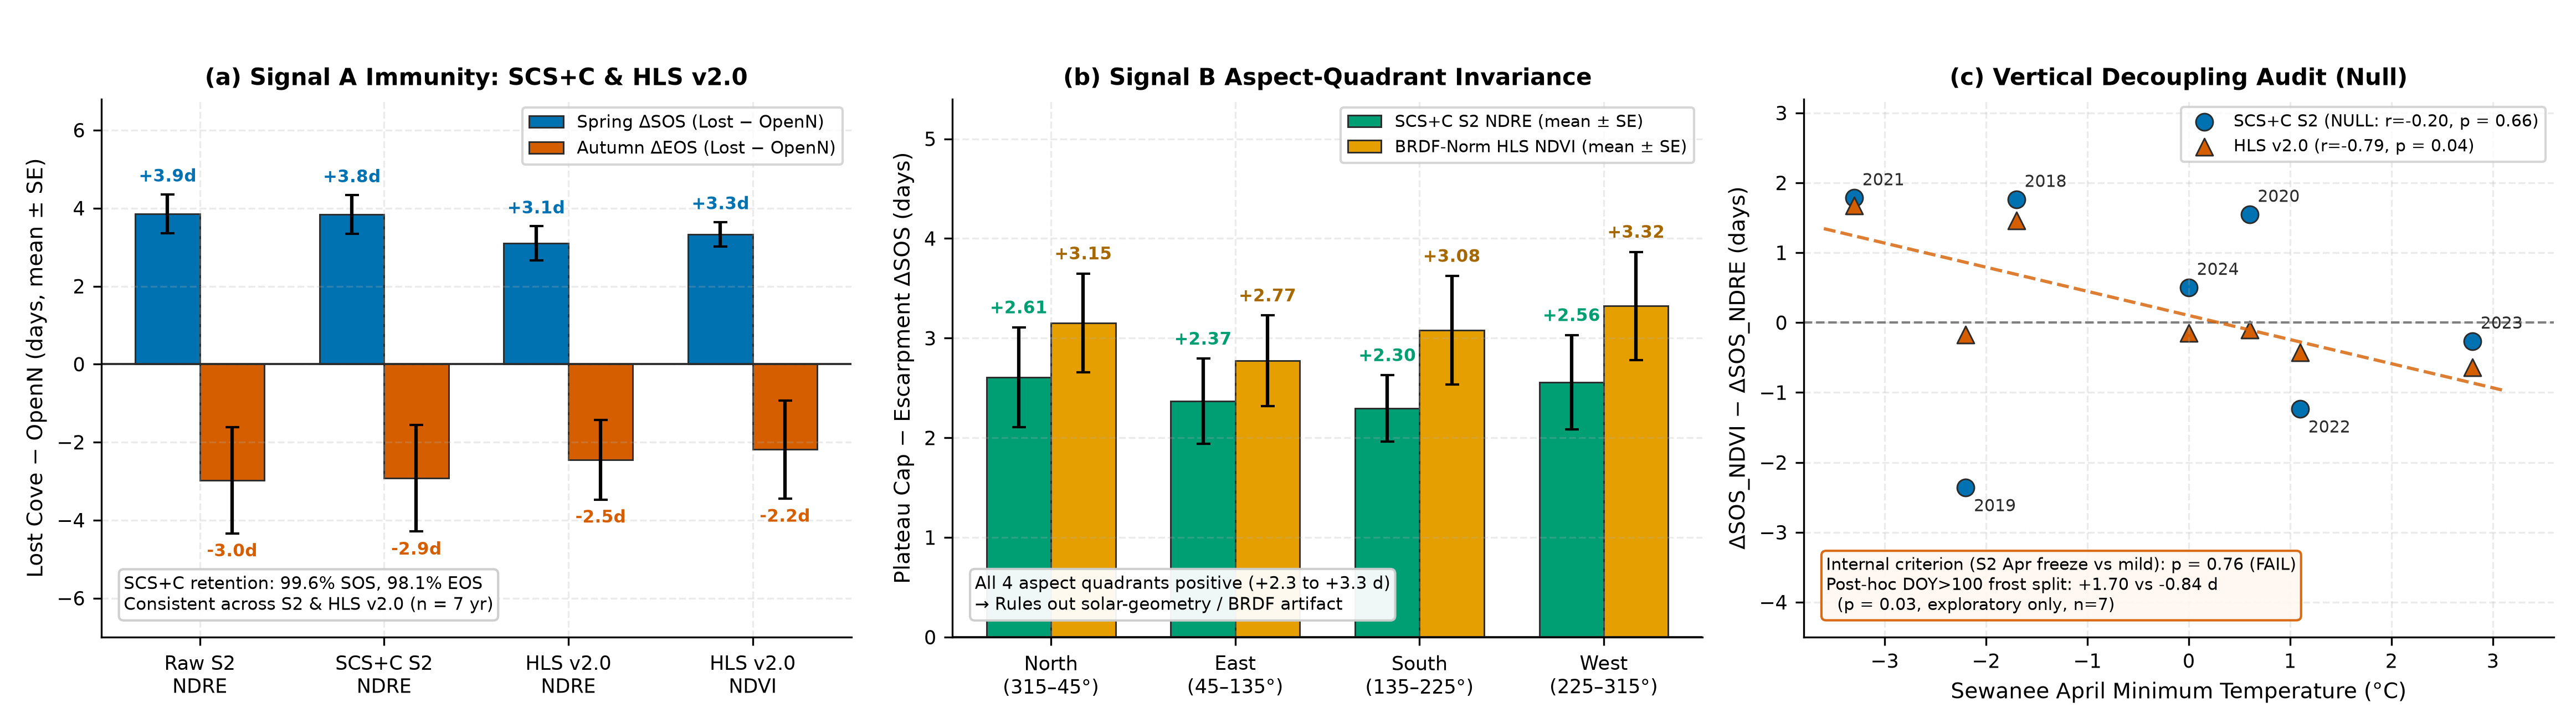
\includegraphics[width=\linewidth]{figures/fig2.png}
\caption{\textbf{Both phenological anomalies survive topographic and BRDF correction, whereas the internal vertical-decoupling test fails.} (a)~Lost Cove minus Open North Cove shifts (mean $\pm$ SE, $n=7$~yr) remain stable across raw Sentinel-2, \texttt{SCS+C} Sentinel-2, and BRDF-normalized NASA \texttt{HLS v2.0}. (b)~Plateau-cap spring delay (Signal~B, mean $\pm$ SE) holds across all four cardinal aspect quadrants, ruling out solar-geometry bias. (c)~Sentinel-2 vertical decoupling ($\Delta\text{SOS}_{\text{NDVI}} - \Delta\text{SOS}_{\text{NDRE}}$) shows no relation to April minimum temperature ($r=-0.20, p=0.66$).}
\label{fig:brdf_decoupling}
\end{figure}

\section{Regional Closed-Karst Cold-Air Pooling Compresses the Growing Season}
\label{sec:regional_karst}

A single valley cannot separate general geomorphic physics from site history. Scanning the Southern Cumberland Plateau with offline Priority-Flood depression filling identified 17 closed basins ($\ge 22.5$~m sill depth, $\ge 0.30~\text{km}^2$). Six basins fell below the 60\% deciduous-floor threshold (\texttt{NLCD-41}) and were excluded prior to regional phenology extraction: \texttt{Karst\_TN\_04} (0\% deciduous, quarry/developed), \texttt{Karst\_TN\_06} (35.4\% 30~m \texttt{NLCD-41}, 58.1\% pasture), \texttt{Karst\_TN\_13} (24.2\% \texttt{NLCD-41}), \texttt{Karst\_AL\_15} (which collapsed to 0~m fill depth at 30~m resolution), \texttt{Lost\_Cove\_TN} (48.7\% 30~m \texttt{NLCD-41}, 38.4\% pasture), and \texttt{Sinking\_Cove\_TN} (57.1\% 30~m \texttt{NLCD-41}). Notably, \texttt{Lost\_Cove\_TN} and \texttt{Sinking\_Cove\_TN} therefore sit outside the 11~regional phenology pairs and later join five of those pairs in the seven-cove \texttt{ECOSTRESS} thermal tile (\cref{sec:thermal_25yr}). The remaining 11 forested closed-karst basins span 170~km from Tennessee into northern Alabama (9 meeting the strict 30~m cutoff of $\text{FillDepth} \ge 25$~m and area $\ge 0.35~\text{km}^2$) and were matched 1:1 with adjacent open-drainage gorges (\cref{tab:karst_census}).

\begin{figure}[t]
\centering
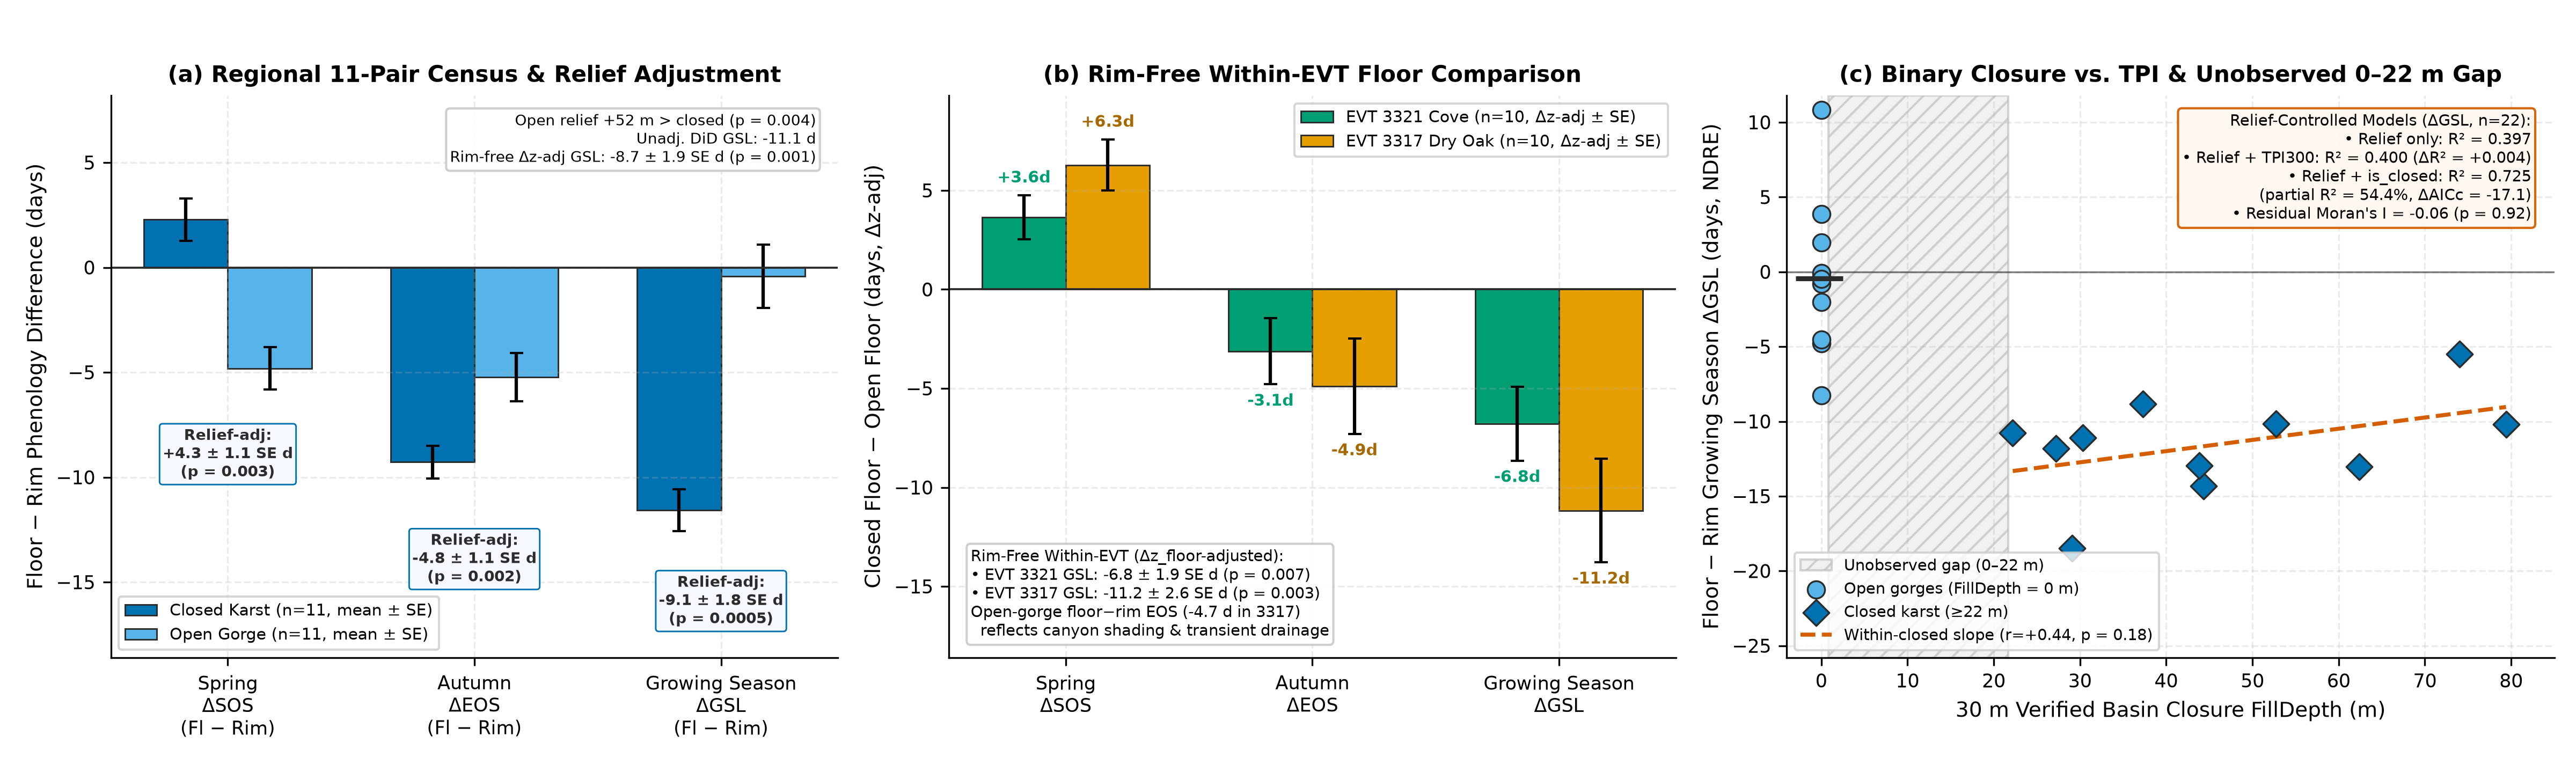
\includegraphics[width=\linewidth]{figures/fig3.png}
\caption{\textbf{Closed karst basins compress growing seasons after relief and rim-free controls.} (a)~Floor-minus-rim NDRE (mean $\pm$ SE) across 11 closed (dark blue) vs.\ 11 open basins (light blue), annotated with relief-adjusted CR1 estimates ($\Delta\text{GSL}=-9.1 \pm 1.8$~d SE, $p=0.0005$). (b)~Rim-free $\Delta z_{\text{floor}}$-adjusted differences persist within identical dry oak (\texttt{EVT 3317}, $-11.2$~d) and cove (\texttt{EVT 3321}, $-6.8$~d) classes. (c)~Binary closure adds 54.4\% partial $R^2$ over relief ($\Delta\text{AIC}_c=-17.1$ vs.\ TPI), with 0--22~m sills unobserved (hatched) and no ramp above 22~m.}
\label{fig:regional_karst}
\end{figure}

\subsection{Relief-Adjusted Inference and Rim-Free Floor-vs-Floor Verification}
Auditing pair geometry revealed a systematic relief imbalance: open-drainage controls have 51.8~m greater floor-to-rim relief than closed basins (mean $178.3 \pm 53.6$~m SD vs.\ $126.5 \pm 41.2$~m SD, paired $p=0.0043$), and 7/11 open rims sit at or above 535~m elevation (where the plateau-cap spring lag operates) compared with 2/11 closed rims. Greater elevation relief alone shifts open floor-minus-rim $\Delta\text{SOS}$ more negative and inflates the unadjusted paired Difference-in-Differences (NDRE unadjusted DiD: $\Delta\text{SOS}=+7.09$~d, $\Delta\text{EOS}=-4.05$~d, $\Delta\text{GSL}=-11.14$~d; NDVI unadjusted $\Delta\text{GSL}=-10.67$~d).

Adjusting 22-site NDRE regressions explicitly for floor-to-rim relief with CR1 pair-clustered standard errors ($\text{df}=10$) confirms a smaller but well-supported growing-season compression (\cref{fig:regional_karst}a, \cref{tab:karst_census}): closed basins delay spring by $+4.28 \pm 1.13$~d (SE, $p=0.0035$), advance autumn by $-4.79 \pm 1.13$~d (SE, $p=0.0017$), and shorten the growing season by $-9.07 \pm 1.81$~d (SE, $p=0.00053$), with no $\text{is\_closed} \times \text{relief}$ interaction ($p=0.66$--$0.86$). NDVI yields a consistent relief-adjusted compression ($\Delta\text{SOS}=+4.20 \pm 1.21$~d SE, $p=0.0059$; $\Delta\text{EOS}=-3.84 \pm 1.26$~d SE, $p=0.012$; $\Delta\text{GSL}=-8.04 \pm 2.10$~d SE, $p=0.0034$), and the strict 30~m nine-pair subset behaves similarly ($\Delta\text{GSL}=-10.20 \pm 2.04$~d SE in NDRE, $p=0.0011$).

To bypass rim elevation and plateau-cap effects altogether, we also compared closed and open \emph{floors} directly while adjusting for residual floor-elevation differences ($\Delta z_{\text{floor}}$, mean $+12.3$~m). Across all 11 pairs in NDRE, rim-free $\Delta z_{\text{floor}}$-adjusted floor-vs-floor regression yields $\Delta\text{SOS}=+5.56 \pm 1.15$~d (SE, $p=0.00095$), $\Delta\text{EOS}=-3.19 \pm 1.38$~d (SE, $p=0.047$), and $\Delta\text{GSL}=-8.75 \pm 1.85$~d (SE, $p=0.0011$). Stratifying floors strictly within identical \texttt{LANDFIRE} ecological types ($n=10$ valid pairs per class, $\Delta z_{\text{floor}}$-adjusted) shows that growing-season compression persists inside both \texttt{EVT 3317} dry oak forest ($\Delta\text{SOS}=+6.28 \pm 1.29$~d SE, $p=0.0012$; $\Delta\text{EOS}=-4.89 \pm 2.41$~d SE, $p=0.077$; $\Delta\text{GSL}=-11.17 \pm 2.61$~d SE, $p=0.0027$) and \texttt{EVT 3321} mesophytic cove forest ($\Delta\text{SOS}=+3.65 \pm 1.10$~d SE, $p=0.011$; $\Delta\text{EOS}=-3.13 \pm 1.67$~d SE, $p=0.098$; $\Delta\text{GSL}=-6.78 \pm 1.87$~d SE, $p=0.0067$; \cref{fig:regional_karst}b). Closed floors contain more dry oak (57.7\% \texttt{EVT 3317}) and less cove forest (25.6\% \texttt{EVT 3321}) than open floors (44.0\% \texttt{EVT 3321}), ruling out mesophytic species enrichment as the cause.

Under internal decision criterion P1, we record the overall status transparently as \texttt{PARTIAL\_PASS}: although every closed basin (11/11) senesces earlier on its floor than its rim ($-9.28 \pm 2.57$~d SD in NDRE) and paired/relief-adjusted tests pass, two sub-criteria failed: open-gorge controls themselves showed $-3.03$~d (NDVI) to $-5.23$~d (NDRE) floor-minus-rim EOS (reflecting canyon shading and transient drainage even within identical \texttt{EVT 3317}, $-4.74$~d, $p=0.0048$), and $r(\sigma_{\text{SOS}}, \text{FillDepth})$ reached 0.22 in NDVI (exceeding the 0.15 internal threshold).

\begin{table}[t]
\centering
\begin{threeparttable}
\caption{\textbf{Regional closed-karst phenology (NDRE, $N=11$ pairs) and relief-controlled geomorphic models.} All $\pm$ values denote SE (CR1 pair-clustered $\text{df}=10$ in Part~A OLS; OLS $\text{df}=n-2$ in rim-free comparisons).}
\label{tab:karst_census}
\footnotesize
\setlength{\tabcolsep}{4.0pt}
\begin{tabularx}{\linewidth}{@{} >{\raggedright\arraybackslash}X c r r r @{}}
\toprule
Estimator / Model & $n$ & Spring $\Delta$SOS (d) & Autumn $\Delta$EOS (d) & $\Delta$GSL (d) \\
\midrule
\multicolumn{5}{@{}l}{\textit{Part A: Closed-Karst vs.\ Open-Gorge Effects (NDRE)}} \\
\textbf{Relief-adj.\ 22-site CR1 OLS (primary)} & 11 pairs & $+4.28 \pm 1.13$ ($0.0035$) & $-4.79 \pm 1.13$ ($0.0017$) & $\mathbf{-9.07 \pm 1.81}$ ($0.0005$) \\
Relief-adj.\ 22-site CR1 OLS (NDVI) & 11 pairs & $+4.20 \pm 1.21$ ($0.0059$) & $-3.84 \pm 1.26$ ($0.012$) & $-8.04 \pm 2.10$ ($0.0034$) \\
Rim-free floor-vs-floor ($\Delta z_{\text{fl}}$-adj.) & 11 pairs & $+5.56 \pm 1.15$ ($0.0010$) & $-3.19 \pm 1.38$ ($0.047$) & $-8.75 \pm 1.85$ ($0.0011$) \\
Within \texttt{EVT 3317} dry oak ($\Delta z_{\text{fl}}$-adj.) & 10 pairs & $+6.28 \pm 1.29$ ($0.0012$) & $-4.89 \pm 2.41$ ($0.077$) & $-11.17 \pm 2.61$ ($0.0027$) \\
Within \texttt{EVT 3321} cove ($\Delta z_{\text{fl}}$-adj.) & 10 pairs & $+3.65 \pm 1.10$ ($0.011$) & $-3.13 \pm 1.67$ ($0.098$) & $-6.78 \pm 1.87$ ($0.0067$) \\
Unadjusted paired DiD (for reference) & 11 pairs & $+7.09 \pm 1.23$ ($0.0002$) & $-4.05 \pm 1.08$ ($0.0038$) & $-11.14 \pm 1.63$ ($4.4{\times}10^{-5}$) \\
\midrule
\multicolumn{5}{@{}l}{\textit{Part B: Relief-Controlled Geomorphic Models Across 22 Sites ($R^2$ and $\text{AIC}_c$ on NDRE $\Delta$GSL)}} \\
Relief only & 22 & \multicolumn{3}{r}{$R^2=0.397$, $\text{AIC}_c=143.5$ ($\Delta\text{AIC}_c=+14.3$ vs.\ best)} \\
Relief + 300~m TPI & 22 & \multicolumn{3}{r}{$R^2=0.400$ ($\Delta R^2=+0.004$), $\text{AIC}_c=146.4$ ($\Delta\text{AIC}_c=+17.1$)} \\
Relief + linear \texttt{FillDepth} & 22 & \multicolumn{3}{r}{$R^2=0.580$, $\text{AIC}_c=138.6$ ($\Delta\text{AIC}_c=+9.3$)} \\
\textbf{Relief + binary \texttt{is\_closed}} & 22 & \multicolumn{3}{r}{$\mathbf{R^2=0.725}$ (partial $R^2=54.4\%$), $\mathbf{\text{AIC}_c=129.3}$ ($\Delta\text{AIC}_c=0.0$)} \\
\bottomrule
\end{tabularx}
\begin{tablenotes}[flushleft]
\footnotesize
\item Parentheses in Part~A give two-sided $p$-values. Internal gate P1 status: \texttt{PARTIAL\_PASS}.
\end{tablenotes}
\end{threeparttable}
\end{table}

\subsection{Binary Topographic Closure vs.\ Local Concavity (0--22~m Unobserved)}
Open gorges and closed karst valleys share nearly identical local concavity (mean 300~m TPI of $-11.5$~m vs.\ $-13.4$~m), so adding 300~m TPI to relief explains virtually no additional variance in NDRE $\Delta\text{GSL}$ ($R^2=0.397$ to $0.400$, $\Delta R^2=+0.004$; \cref{tab:karst_census}). Adding binary topographic closure (\texttt{is\_closed}) lifts $R^2$ from $0.397$ to $0.725$ (partial $R^2=54.4\%$ over relief; $\Delta\text{AIC}_c=-17.1$ relative to relief plus 300~m TPI and $-14.3$ relative to relief alone), with negligible spatial autocorrelation in residuals (permutation Moran's $I=-0.06, p=0.92$).

Importantly, this is a binary closure contrast rather than a continuous depth-response curve (\cref{fig:regional_karst}c). Because all 11 open gorges have $\text{FillDepth}=0$~m and all 11 closed basins have 30~m $\text{FillDepth}$ between 22.2 and 79.4~m, a 25~m saturating hinge equals $25 \times \text{is\_closed}$ on 21/22 sites ($\Delta\text{AIC}_c=0.03$). Within the 11 closed basins above 22~m, deeper 30~m sills do not intensify compression ($r(\Delta\text{EOS}, \text{FillDepth})=+0.26, p=0.45$; $r(\Delta\text{GSL}, \text{FillDepth})=+0.44, p=0.18$), and the shallow 0--22~m sill regime remains unobserved in this regional sample.

\section{ECOSTRESS Thermal Verification and 25-Year Landsat Panel}
\label{sec:thermal_25yr}

Optical phenology alone cannot directly observe cold-air pooling. Merging NASA \texttt{ECOSTRESS} Collection~2 (2020--2024, 144 granules) with Bayesian cloud-masked Collection~3 (2018--2019 and 2025--2026) yields 157 unique in-swath nighttime passes over Sewanee, of which 60 pass standard cloud and QA flags. Auditing those 60 scenes against co-located ERA5-Land 2~m air temperature uncovered 8 unflagged \texttt{ECOv002} anomalies ($|\text{LST}-\text{ERA5}_{t2m}| > 10^\circ$C; 0/14 clean \texttt{v003} scenes affected): seven cloud-contaminated passes reading $11$--$22^\circ$C colder than surface air temperature (including all three scenes with $u_{10} \ge 3.0$~m/s) and one calibration-corrupted pre-dawn pass reading $+46$--$48^\circ$C. Applying a physical $|\text{LST}-\text{ERA5}_{t2m}| \le 10^\circ$C filter retains $n=52$ clean nights ($38$ \texttt{v002}, $14$ \texttt{v003}; $51$ with matched ERA5 wind, as one November 2026 \texttt{v003} scene precedes ERA5 publication; \cref{fig:ecostress_thermal}).

\begin{figure}[t]
\centering
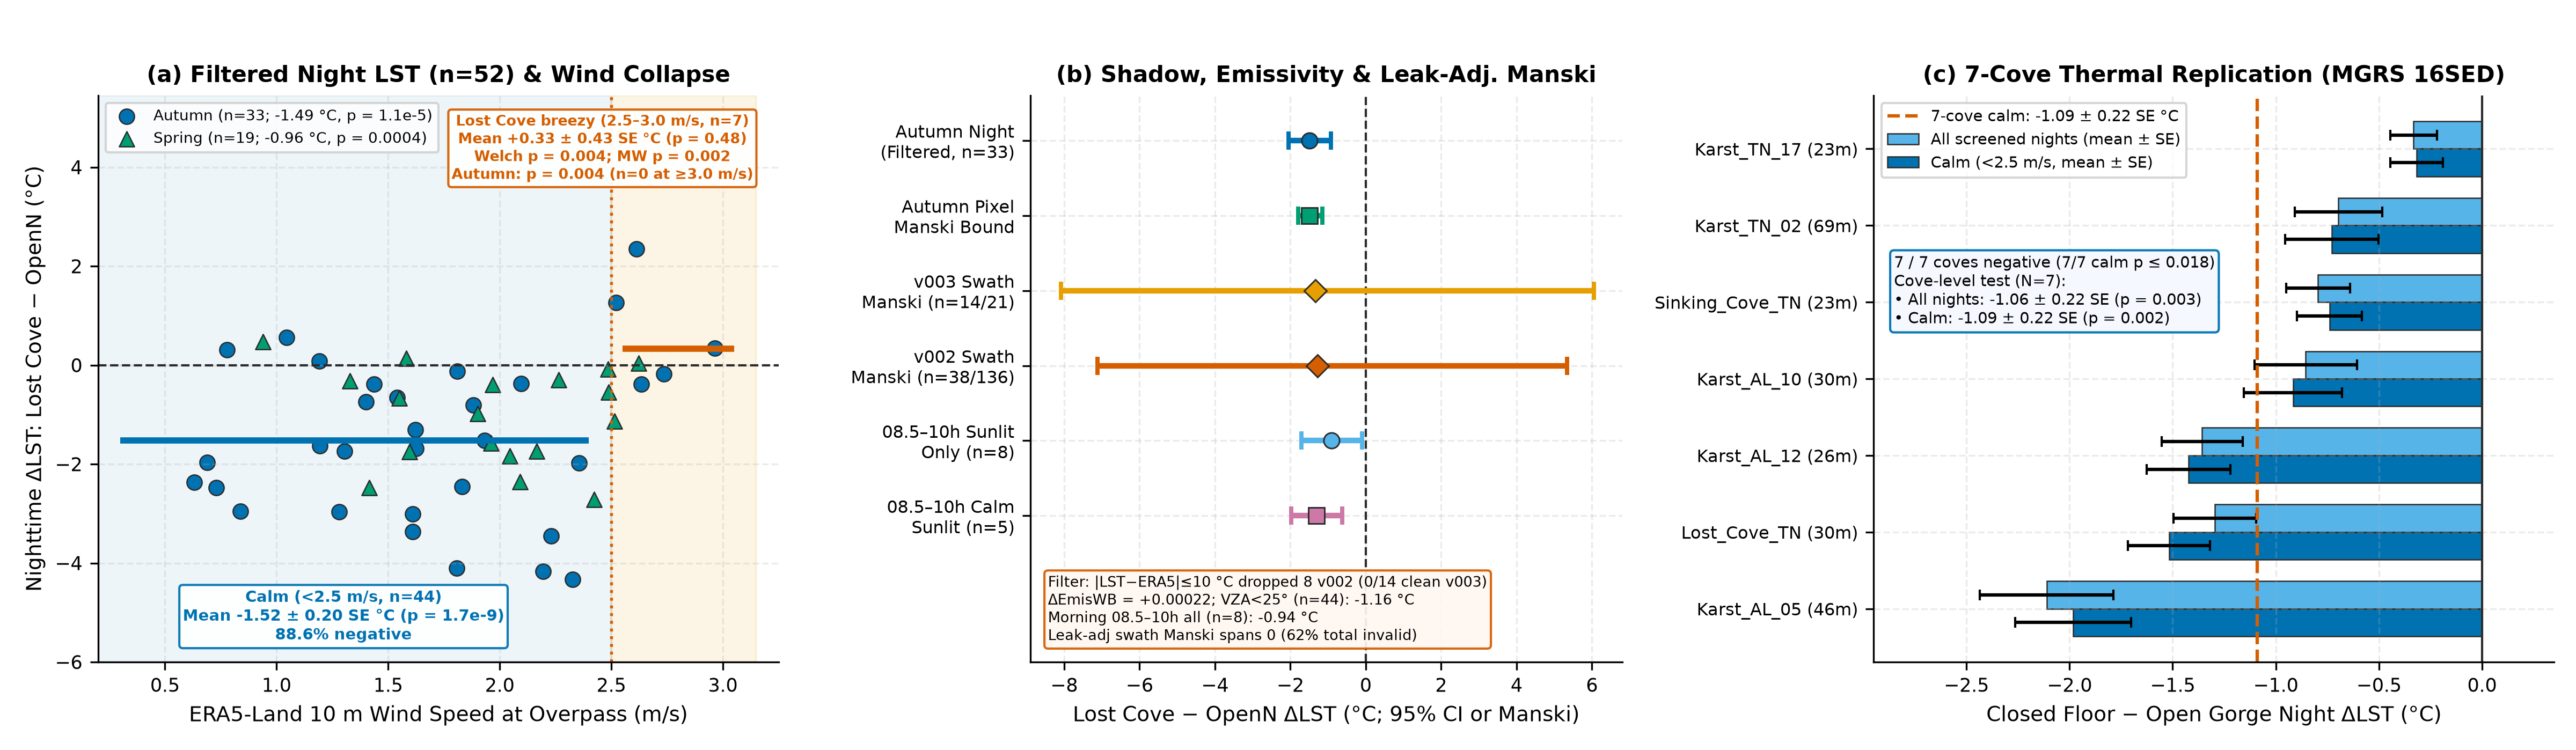
\includegraphics[width=\linewidth]{figures/fig4.png}
\caption{\textbf{Filtered ECOSTRESS confirms nocturnal cooling in spring, autumn, and 7/7 coves.} (a)~Across 52 filtered nights ($|\text{LST}-\text{ERA5}_{t2m}| \le 10^\circ$C), Lost Cove cools in autumn ($-1.49^\circ$C) and spring ($-0.96^\circ$C) under calm winds ($<2.5$~m/s, $-1.52^\circ$C) but collapses over 2.5--3.0~m/s ($+0.33^\circ$C, Welch $p=0.004$). (b)~Controls show negligible emissivity bias ($+0.00022$), calm sunlit morning cooling ($-1.30^\circ$C), negative pixel bounds, and leak-adjusted \texttt{v002}/\texttt{v003} swath Manski bounds spanning zero. (c)~All 7/7 closed basins in tile \texttt{16SED} run colder than open gorges ($-1.09 \pm 0.22^\circ$C SE calm).}
\label{fig:ecostress_thermal}
\end{figure}

Removing the eight corrupted \texttt{ECOv002} scenes clarifies seasonal cooling in Lost Cove relative to elevation-matched Open North Coves. Whereas the unfiltered spring parametric test was distorted by four cloud-leaked passes ($n=23$, mean $-0.37^\circ$C, $p=0.42$), filtered spring nights (February--April, $n=19$) average $-0.96 \pm 0.22^\circ$C (SE, median $-0.67^\circ$C, 84.2\% negative, $t$-test $p=0.00042$, Wilcoxon $p=0.00034$; calm spring $n=17$: $-1.01 \pm 0.24^\circ$C SE, $p=0.00072$). Autumn nights (September--November, $n=33$) average $-1.49 \pm 0.29^\circ$C (SE, median $-1.63^\circ$C, $t$-test $p=1.1 \times 10^{-5}$, Wilcoxon $p=1.0 \times 10^{-5}$; October $n=7$: $-2.07 \pm 0.65^\circ$C SE, $p=0.019$). Across all 52 filtered nights, Lost Cove averages $-1.30 \pm 0.20^\circ$C (SE, $p=3.8 \times 10^{-8}$).

Boundary-layer cold pools should erode once wind mixes the valley atmosphere \citep{whiteman1982}. At Lost Cove, calm nights ($u_{10}<2.5$~m/s, $n=44$) average $-1.52 \pm 0.20^\circ$C (SE, $p=1.7 \times 10^{-9}$, 88.6\% negative), whereas breezy nights ($2.5 \le u_{10} < 3.0$~m/s, $n=7$) shift to $+0.33 \pm 0.43^\circ$C (SE, $p=0.48$; Welch $p=0.0041$, Mann-Whitney $p=0.0019$; season-controlled OLS $\beta=+1.90 \pm 0.52^\circ$C SE, $p=0.00065$; \cref{fig:ecostress_thermal}a). Within autumn alone, calm nights ($n=27, -1.84 \pm 0.27^\circ$C SE) separate cleanly from breezy nights ($n=5, +0.68 \pm 0.51^\circ$C SE; Welch $p=0.0038$, Mann-Whitney $p=0.0015$). Two scope limits apply: zero clean scenes occur at $u_{10} \ge 3.0$~m/s (continuous linear slope across $0.5$--$3.0$~m/s is $r=0.11, p=0.46$, consistent with a regime threshold rather than a linear trend), and wind collapse does not replicate across the six other \texttt{16SED} coves when using Sewanee's point ERA5 wind (paired calm vs.\ breezy $p=0.77$), likely reflecting spatial wind decorrelation 30--90~km south of Sewanee and deeper basin shelter.

Within MGRS tile \texttt{16SED} (single-tile spatial scope), restricting multi-cove analysis to \texttt{v002} granules verified clear over Sewanee ($|\text{LST}-\text{ERA5}_{t2m}| \le 10^\circ$C, excluding 10 Sewanee-flagged leak granules and 16 cloudy-at-Sewanee passes) shows that all 7/7 closed karst basins replicate calm-night cooling individually on both parametric and Wilcoxon tests (\cref{fig:ecostress_thermal}c): \texttt{Lost\_\allowbreak Cove\_TN} ($n=44, -1.52 \pm 0.20^\circ$C SE, $t$ $p=1.7 \times 10^{-9}$, Wilc.\ $p=1.2 \times 10^{-7}$), \texttt{Karst\_\allowbreak AL\_05} ($n=30, -1.98 \pm 0.28^\circ$C SE, $t$ $p=9.4 \times 10^{-8}$, Wilc.\ $p=6.9 \times 10^{-7}$), \texttt{Karst\_\allowbreak AL\_12} ($n=22, -1.42 \pm 0.20^\circ$C SE, $t$ $p=6.0 \times 10^{-7}$, Wilc.\ $p=4.8 \times 10^{-6}$), \texttt{Karst\_\allowbreak AL\_10} ($n=30, -0.92 \pm 0.24^\circ$C SE, $t$ $p=0.00059$, Wilc.\ $p=0.00035$), \texttt{Sinking\_\allowbreak Cove\_TN} ($n=32, -0.74 \pm 0.16^\circ$C SE, $t$ $p=5.3 \times 10^{-5}$, Wilc.\ $p=9.7 \times 10^{-5}$), \texttt{Karst\_\allowbreak TN\_02} ($n=34, -0.73 \pm 0.23^\circ$C SE, $t$ $p=0.0030$, Wilc.\ $p=5.8 \times 10^{-7}$), and \texttt{Karst\_\allowbreak TN\_17} ($n=33, -0.32 \pm 0.13^\circ$C SE, $t$ $p=0.018$, Wilc.\ $p=0.019$), yielding a cove-level calm mean of $-1.09 \pm 0.22^\circ$C (SE, $N=7, p=0.0024$; all screened nights $-1.06 \pm 0.22^\circ$C SE, $p=0.0029$). Artifact checks show negligible emissivity differences ($\Delta\text{EmisWB}=+0.00022$, $<0.02^\circ$C bias), consistent cooling at low view angles ($\text{VZA}<25^\circ, n=44: -1.16 \pm 0.20^\circ$C SE, $p=9.1 \times 10^{-7}$), and persistent calm sunlit morning cooling at 08:30--10:00 solar time ($n=5, -1.30 \pm 0.35^\circ$C SE, $p=0.020$; all $n=8$ morning passes $-0.94 \pm 0.41^\circ$C SE, $p=0.055$, despite $+5.2\%$ higher ray-traced direct morning insolation in Lost Cove; \cref{fig:ecostress_thermal}b).

Despite consistent clear-sky cooling, thermal remote sensing carries an important censoring bound. Clean-scene pixel \citet{manski1990} bounds stay strictly negative ($[-1.79, -1.15]^\circ$C in autumn; $[-1.50, -1.08]^\circ$C overall). At the swath level, properly treating all unflagged cloud-leaked passes ($|\text{LST}-\text{ERA5}_{t2m}| > 10^\circ$C: 9 in \texttt{v002} and 3 non-clean passes in \texttt{v003}) as unobserved yields worst-case bounds spanning zero in both \texttt{v002} ($n=38/136$ clean, 29.8\% leak-adjusted vs.\ 24.1\% raw cloud-flagged, $[-7.12, +5.34]^\circ$C) and \texttt{v003} ($n=14/21$ clean, 23.8\% leak-adjusted vs.\ 10.9\% raw cloud-flagged, $[-8.09, +6.05]^\circ$C), as well as across all 157 combined passes (29.0\% leak-adjusted cloud missingness $[-8.12, +6.28]^\circ$C; total invalid fraction 62.0\% vs.\ 63.3\%, $[-15.93, +14.95]^\circ$C). Although differential missingness between Lost Cove and Open North Coves is small ($<1.3\%$), closing the worst-case fog bound requires ground temperature loggers.

\subsection{25-Year Landsat Persistence, Sensor Limits, and Falsification of P4}
Across 25 years of Roy-harmonized Landsat 5--9 (2000--2024), Lost Cove greens up later than Open North Coves in 88\% of springs (median $+2.45$~d) and senesces earlier in 80\% of autumns (median $-2.53$~d; \cref{fig:landsat_25yr}a). Two sparse-observation outlier years (2007 EOS $+23.6$~d; 2013 SOS $-30.8$~d) widen variance so that unscreened 25-year OLS means are not statistically significant ($\Delta\text{SOS}=+1.62 \pm 1.42$~d SE, $p=0.27$; $\Delta\text{EOS}=-2.22 \pm 1.34$~d SE, $p=0.11$; net $\Delta\text{GSL}=-3.83$~d, or $-5.98$~d excluding 2007 and 2013). Cross-sensor validation against \texttt{HLS v2.0} over 2018--2024 reveals an asymmetric precision limit: 16-day Landsat reproduces interannual autumn $\Delta\text{EOS}$ closely ($r=0.961, p=0.00056$), but fails to track interannual spring $\Delta\text{SOS}$ ($r=-0.041, p=0.93$).

\begin{figure}[t]
\centering
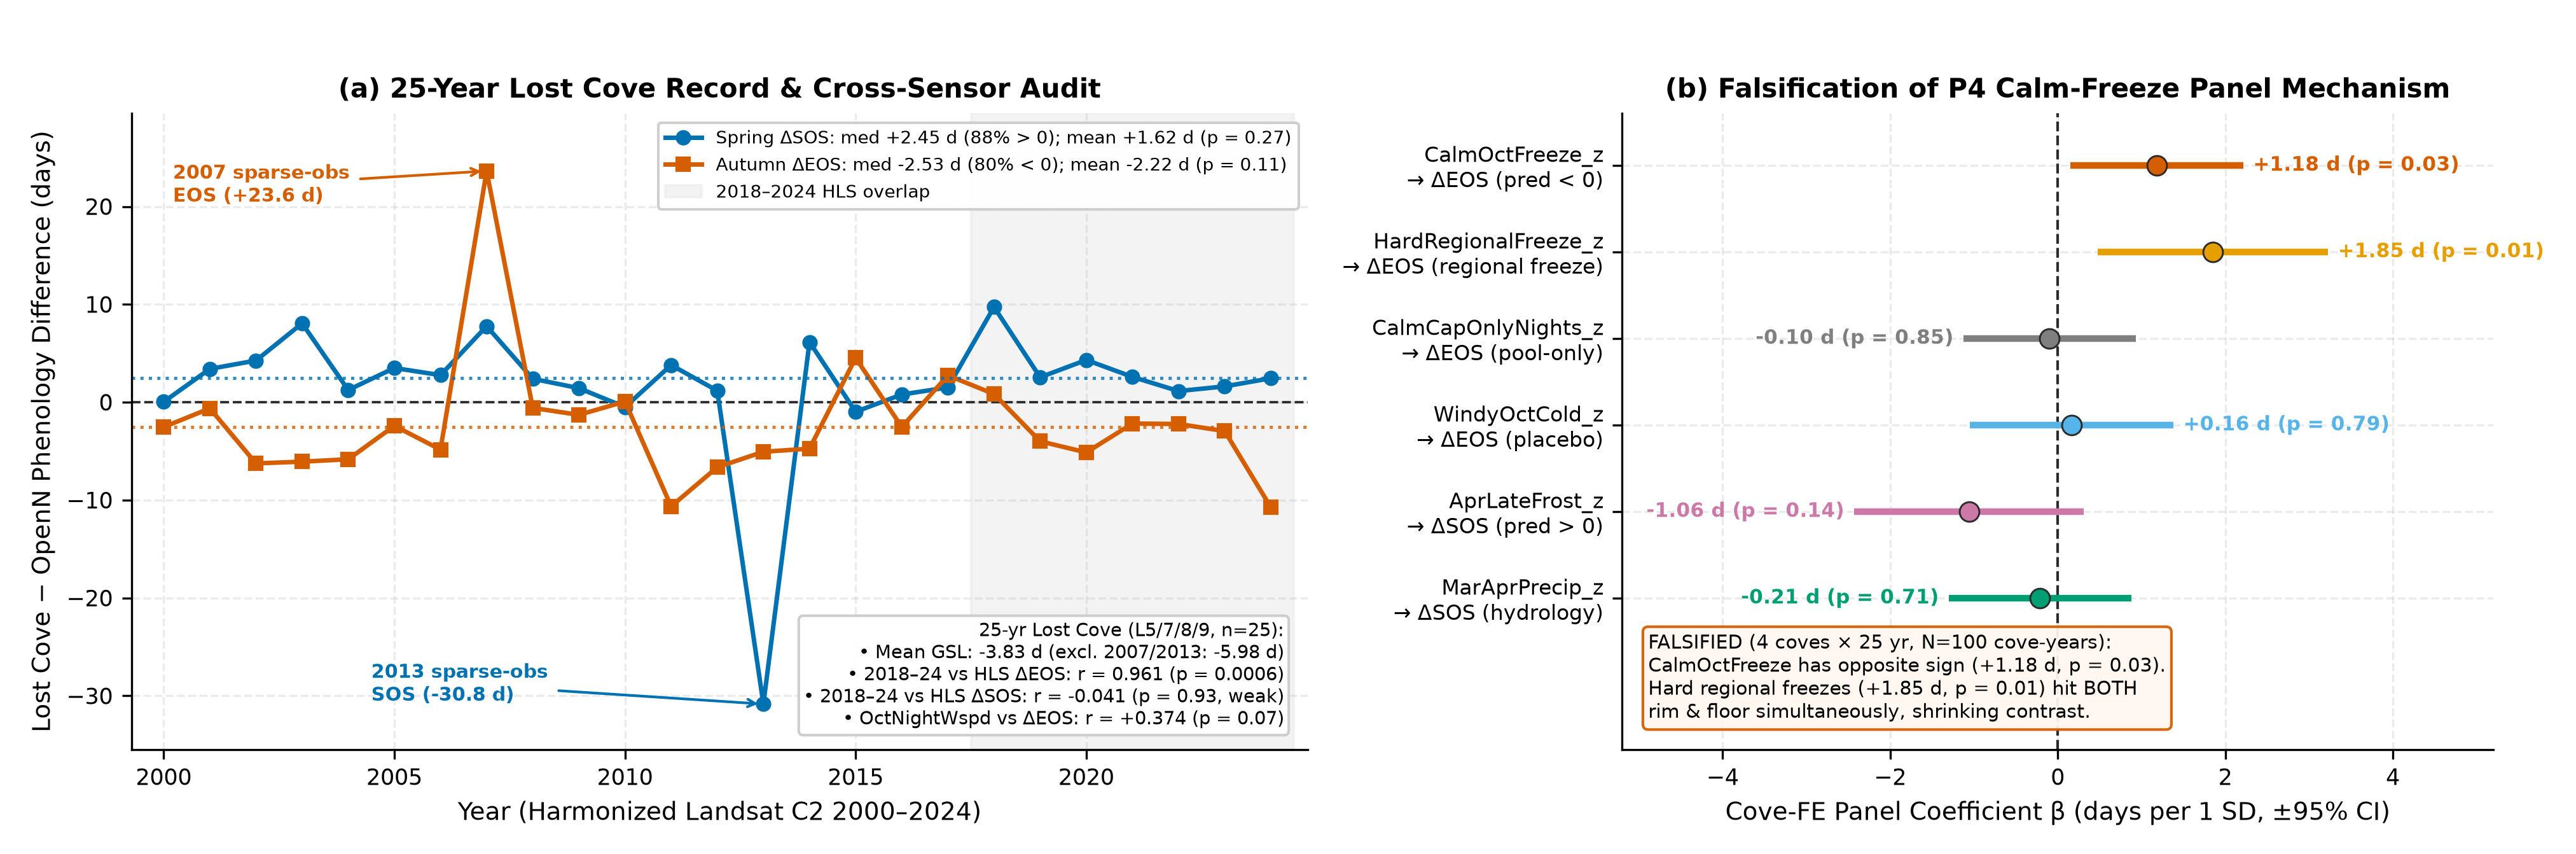
\includegraphics[width=\linewidth]{figures/fig5.png}
\caption{\textbf{25-year Landsat persistence, spring cross-sensor limits, and falsification of P4.} (a)~Harmonized Landsat (2000--2024) records positive spring $\Delta\text{SOS}$ in 88\% of years (median $+2.45$~d, OLS mean $p=0.27$) and negative autumn $\Delta\text{EOS}$ in 80\% (median $-2.53$~d, OLS mean $p=0.11$); over 2018--2024 it tracks \texttt{HLS v2.0} in autumn ($r=0.961, p=0.0006$) but not spring ($r=-0.041, p=0.93$). (b)~Four-cove $\times$ 25-year panel coefficients ($\pm 95\%$ CI): \texttt{CalmOctFreeze} flips positive ($+1.18$~d, $p=0.035$) because hard regional freezes ($+1.85$~d) affect rims and floors together.}
\label{fig:landsat_25yr}
\end{figure}

Our internal four-cove $\times$ 25-year fixed-effects panel test (P4, $N=100$ cove-years) predicted that more calm October freeze nights would make floor-minus-rim $\Delta\text{EOS}$ more negative. The data falsified this prediction with the opposite sign ($\beta=+1.18 \pm 0.53$~d/SD SE, $p=0.035$; \cref{fig:landsat_25yr}b). Decomposing October nights shows that hard regional freezes ($\beta=+1.85 \pm 0.70$~d/SD SE, $p=0.014$) push both upper rims and basin floors below freezing together, compressing the floor--rim contrast, while marginal pool-only nights ($\beta=-0.10 \pm 0.52$~d/SD SE, $p=0.85$) and windy cold placebos ($\beta=+0.16 \pm 0.62$~d/SD SE, $p=0.79$) are indistinguishable from zero. Likewise, nighttime October wind speed (\texttt{OctNightWspd}) is non-significant in Lost Cove ($r=0.37, p=0.065$; daily wind $r=0.44, p=0.027$ is unconfirmed in the 4-cove panel). At 16-day Landsat revisit precision, closed-karst compression therefore appears as a chronic structural microclimate effect rather than a single-storm interannual toggle.

\section{Plateau-Cap Spring Lag: Modeled Soil Null and Guild Evidence}
\label{sec:plateau_guild}

At the upper margin of the escarpment, spring green-up steps sharply later onto the flat sandstone tableland (\cref{fig:hopkins_decomp}a). Stratified comparisons show this lag does not stem simply from crossing the 547~m limestone--sandstone lithologic contact: holding steep slope constant ($>10^\circ$, 507~m to 566~m) in \texttt{SCS+C} NDRE shifts spring by $+3.11 \pm 0.53$~d (SE, $n=7$~yr) and autumn by $-3.34 \pm 0.41$~d (SE; \texttt{HLS v2.0} NDRE $+3.12$ / $-3.05$~d). Above the sandstone contact ($\ge 550$~m), flat plateau benches ($\le 8^\circ$, mean elevation 575.4~m) lag adjacent steep rocky rims ($>10^\circ$, mean 566.8~m) by $+3.53$~d across just $+8.62$~m of elevation ($+3.31$~d inside \texttt{EVT 3317} alone). Flat and steep plateau canopies share nearly identical winter NDVI ($0.416$ vs.\ $0.427$), ruling out evergreen understory contamination.

\begin{figure}[t]
\centering
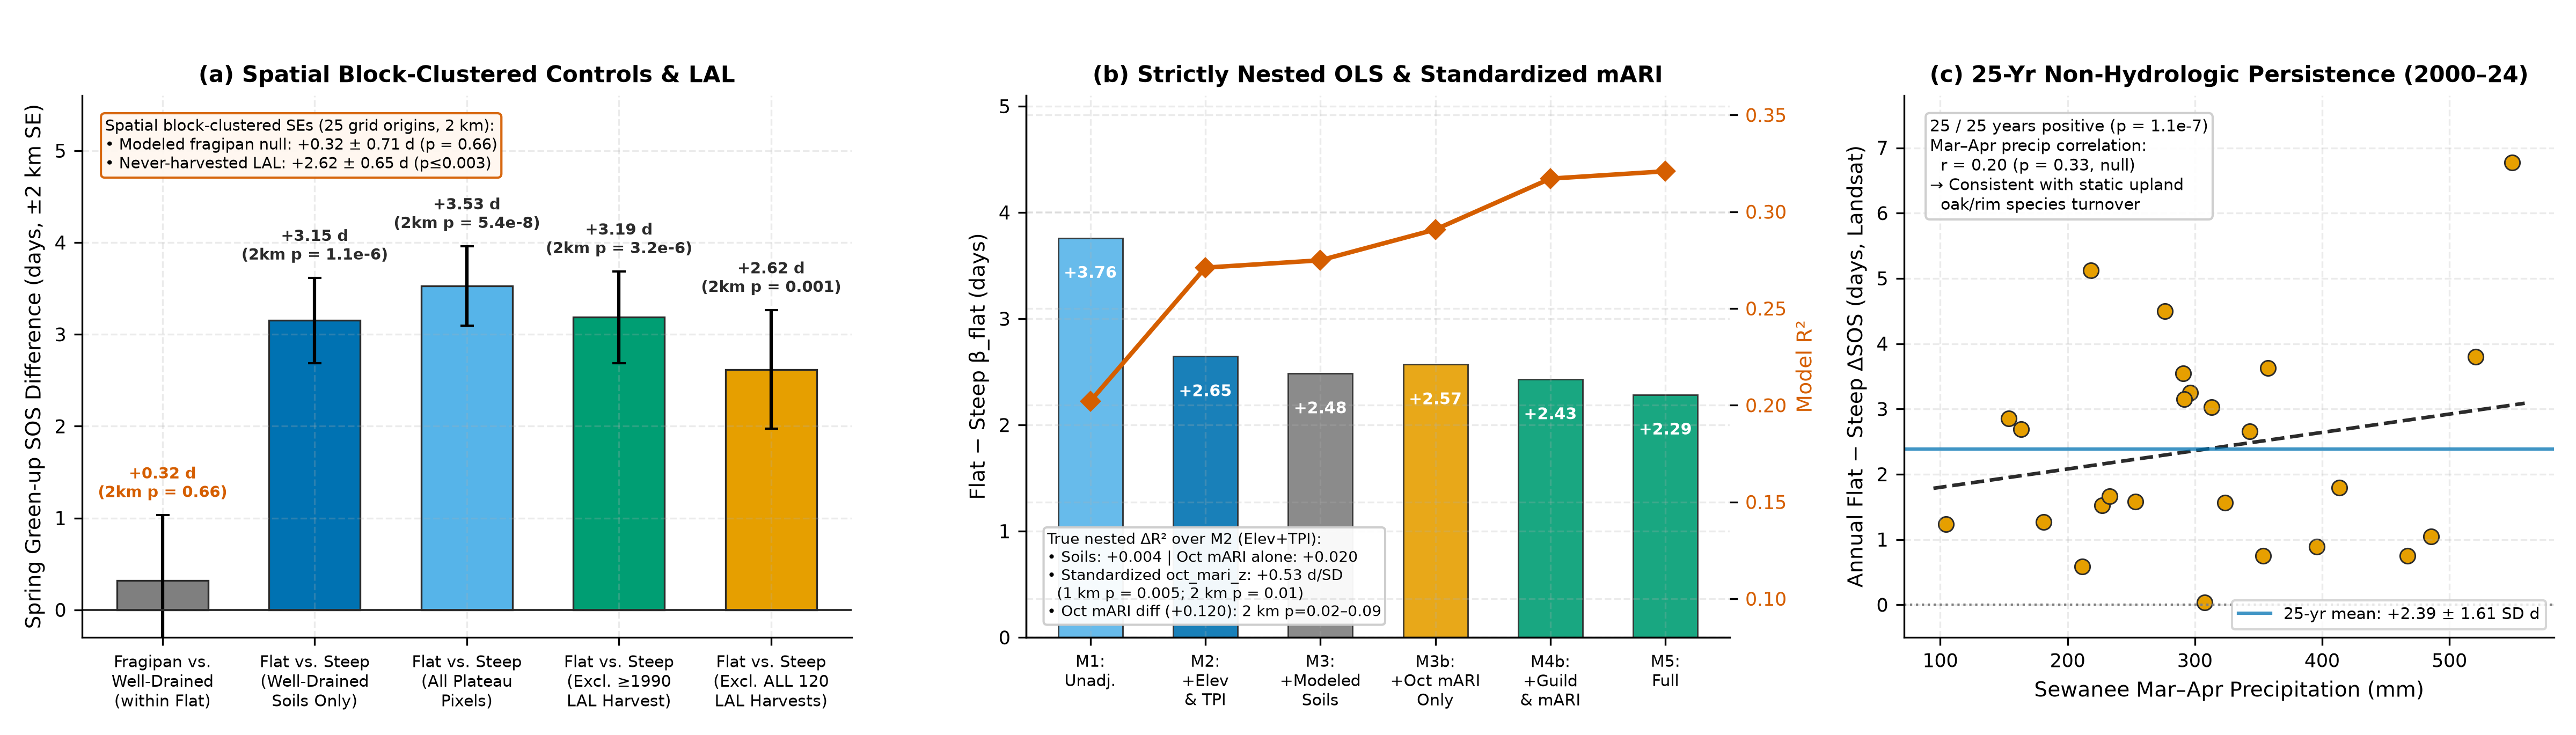
\includegraphics[width=\linewidth]{figures/fig6.png}
\caption{\textbf{Spatial block-clustered tests rule out modeled fragipan inertia and are consistent with plateau-cap guild turnover.} (a)~Multi-origin 2~km spatial block-clustered estimates (mean $\pm$ median 2~km SE across 25 grid origins): within-flat fragipan shows zero delay ($+0.32 \pm 0.71$~d, $p=0.66$), whereas well-drained ($+3.15$~d) and never-harvested LAL stands ($+2.62$~d) remain significant ($p \le 0.0032$). (b)~Strictly nested OLS shows modeled soils add $\Delta R^2=+0.004$, while standardized October \texttt{mARI} enters at $+0.53$~d/SD ($\Delta R^2=+0.020$ alone). (c)~Flat stands lag in 25/25 Landsat years ($+2.39 \pm 1.61$~d SD) with no spring precipitation trend ($r=0.20, p=0.33$).}
\label{fig:plateau_guild}
\end{figure}

Two mechanisms competed under internal criterion P5: (i)~\emph{pedological thermal inertia}, wherein dense subsurface fragipans on flat benches perch cold spring rainwater and delay root warming, and (ii)~\emph{upland oak guild turnover}, wherein level fire-prone sandstone uplands favor late-leafing ring-porous oaks and hickories (\emph{Quercus coccinea}, \emph{Q.\ alba}, \emph{Q.\ montana}) over earlier-flushing mesophytes (\emph{Liriodendron tulipifera}, \emph{Acer rubrum}) sheltered along steep rocky rims. Because 30~m pixels are spatially autocorrelated, we evaluate all plateau-cap contrasts using CR1 spatial block-clustered standard errors across 25 multi-origin grid alignments at both 1~km and 2~km block sizes rather than unclustered pixel $p$-values (\cref{fig:plateau_guild}a).

Modeled soil inertia is falsified across every check. Within the flat plateau cap ($n=700$~pixels), \texttt{gNATSGO}/SSURGO fragipan or poorly drained soils differ from well-drained Hartsells and Ramsey soils by only $+0.32$~d (1~km median SE $= 0.76$~d, $p=0.64$--$0.74$; 2~km median SE $= 0.71$~d, $p=0.55$--$0.74$, 0\% of grid origins $<0.05$). Adding 30~m \texttt{POLARIS} hydraulic conductivity, clay, and bulk-density layers \citep{chaney2019} plus \texttt{gNATSGO} fragipan indicators to an elevation-and-TPI baseline (M2) raises $R^2$ by only $+0.0038$ ($0.271$ to $0.275$; \cref{fig:plateau_guild}b). Over 25 Landsat years (2000--2024), flat benches lag steep rims in 25/25 years ($+2.39 \pm 1.61$~d SD, one-sample $p=1.1 \times 10^{-7}$), with no correlation to March--April precipitation ($r=0.20, p=0.33$; \cref{fig:plateau_guild}c). Because \texttt{POLARIS} and \texttt{gNATSGO} are smoothed modeled soil products, this null falsifies mapped fragipan inertia while leaving unmapped fine-scale edaphic effects possible.

By contrast, four lines of evidence are \emph{consistent with} upland oak guild turnover. First, holding mapped well-drained soils constant ($n=1{,}199$), flat benches still lag steep rims by $+3.15$~d across all 25 spatial block origins (1~km median SE $= 0.39$~d, $p \le 4.5 \times 10^{-9}$; 2~km median SE $= 0.47$~d, $p \le 7.1 \times 10^{-6}$). Second, masking all 120 public Sewanee LAL harvest polygons reduces the raw lag by $\sim 0.9$~d (reflecting silvicultural history) yet leaves $+2.62$~d on never-harvested stands ($n=435$; 1~km median SE $= 0.56$~d, $p \le 0.00063$; 2~km median SE $= 0.65$~d, $p \le 0.0032$, 100\% of origins $<0.01$). Third, the flat-vs-steep lag replicates across all three regional escarpment sites with $\ge 550$~m plateau caps in our archived four-cove dataset: Sewanee ($+2.66$~d, $n=230/38$), Fiery Gizzard ($+2.39$~d, $n=244/15$), and Savage Gulf ($+4.09$~d, $n=218/31$). Fourth, flat plateau canopies exhibit higher October Modified Anthocyanin Reflectance Index (\texttt{mARI}, \citealp{gitelson2001}; $+0.120$), characteristic of red-foliage upland oaks: in strictly nested regressions, standardized \texttt{oct\_mari\_z} enters at $+0.53$~d per SD (1~km median SE $= 0.18$~d, $p=0.0011$--$0.015$; 2~km median SE $= 0.19$~d, $p=0.0015$--$0.065$, 84\% of origins $<0.05$) and adds true single-variable $\Delta R^2=+0.020$ over M2 (full guild plus \texttt{mARI} adds $+0.046$). Notably, the unadjusted flat-vs-steep \texttt{oct\_mari} difference ($+0.120$) is grid-alignment-sensitive at 2~km clustering ($p=0.017$--$0.094$, 36\% of origins $<0.05$; 1~km $p=0.012$--$0.036$). Because no ground species tallies were collected, we interpret these patterns as consistent with---rather than direct plot-level proof of---upland oak guild turnover.

\begin{table}[t]
\centering
\begin{threeparttable}
\caption{\textbf{Complete internal decision-criteria ledger (H1--H7), reporting exact verdicts including partial passes and falsified predictions.}}
\label{tab:hypothesis_ledger}
\small
\begin{tabularx}{\linewidth}{@{} l l >{\raggedright\arraybackslash}X @{}}
\toprule
ID & Status & Key Quantitative Evidence (All $\pm$ Labeled) \\
\midrule
H1 & \textbf{Supported} & MODIS 50\% \texttt{MidGreenup\_1} $= 3.19 \pm 0.17$~d/100~m SE (Hopkins $= 3.28$, trend $p=0.86$); 3-factor decomposition attributes $-0.80$~d/100~m to 50\% vs.\ 15\% metric ($+0.01$ QA/NLCD); Landsat 2013 step non-identifiable ($p=0.91$). \\
H2 & \textbf{Partial/Fail} & \texttt{SCS+C} retains 99.6\% SOS / 98.1\% EOS; Signal~B aspect-invariant ($+2.30$ to $+3.32$~d) and survives unlogged stands ($+2.62$~d, 2~km $p \le 0.0032$). Internal gate P2 recorded as \texttt{PARTIAL\_OR\_FAIL}. \\
H3 & \textbf{Partial Pass} & 11 pairs (NDRE): relief-adj.\ CR1 $\Delta\text{GSL}=-9.07 \pm 1.81$~d SE ($p=0.00053$); rim-free $\Delta z$-adj.\ $-8.75 \pm 1.85$~d SE ($p=0.0011$); persists in \texttt{EVT 3317} ($-11.2$~d) and \texttt{3321} ($-6.8$~d); binary closure partial $R^2=54.4\%$ over relief (0--22~m unobserved). P1 \texttt{PARTIAL\_PASS}. \\
H4 & \textbf{Supported$^*$} & 52 cloud-leak-filtered \texttt{ECOSTRESS} nights (8 \texttt{v002} leaks dropped): spring $-0.96 \pm 0.22^\circ$C SE ($p=0.00042$), autumn $-1.49 \pm 0.29^\circ$C SE ($p=1.1{\times}10^{-5}$); Lost Cove wind collapse over 2.5--3.0~m/s ($p=0.0041$); 7/7 \texttt{16SED} coves individually $p \le 0.018$ ($-1.09 \pm 0.22^\circ$C SE). $^*$Leak-adjusted swath Manski bounds span 0. \\
H5 & \textbf{Split} & Modeled fragipan inertia \textbf{falsified} ($+0.32 \pm 0.71$~d 2~km SE, $p=0.66$; 25-yr precip $r=0.20$). Consistent with oak guild turnover ($+3.15$~d well-drained, 25/25~yr $+2.39$~d, \texttt{oct\_mari\_z} $+0.53$~d/SD, 2~km \texttt{mARI} diff grid-sensitive). \\
H6 & \textbf{Falsified} & Internal S2 April-freeze vertical decoupling failed ($r=-0.20, p=0.66$; freeze vs.\ mild $p=0.76$). HLS $r=-0.79$ and post-DOY-100 split ($p=0.025$) are exploratory only. \\
H7 & \textbf{Falsified} & 25-yr 4-cove \texttt{CalmOctFreeze} panel showed \emph{opposite} sign ($\beta=+1.18 \pm 0.53$~d/SD SE, $p=0.035$) as hard regional freezes ($\beta=+1.85$~d/SD) affect rims and floors together. \\
\bottomrule
\end{tabularx}
\end{threeparttable}
\end{table}

\section{Discussion, Limitations, and Priority Field Measurements}
\label{sec:discussion}

\subsection{Positioning Against Prior Satellite Studies of Hopkins' Law and Cold-Air Pooling}
More than a century after \citet{hopkins1918} proposed his 3.28~d/100~m rule, our results clarify when linear elevation scaling holds and where tableland geomorphology bends it. Along open slopes of the Southern Cumberland Plateau, deciduous 50\% \texttt{MODIS MidGreenup\_1} averages $3.19 \pm 0.17$~d/100~m (SE), matching Hopkins' rate and aligning with continental PhenoCam syntheses \citep{richardson2019} and satellite altitudinal growing-season analyses in southwest China \citep{jiang2022}. Our three-factor MODIS decomposition also cautions against calling steeper 15\% onset slopes ($3.98$~d/100~m) an artifact: early onset and mid-greenup represent distinct canopy phases whose elevational sensitivities differ by $0.80$~d/100~m even under identical deciduous and QA masks.

For cold-air pooling, our contribution is incremental over \citet{mizuno2026}, who demonstrated phenological reversal using HLS and nighttime thermal imagery inside a single Japanese basin, and complements ground-sensor evidence that cold-air pooling filters temperate forest composition \citep{pastore2024} as well as earlier single-valley satellite studies \citep{fisher2006, elmore2012, ward2018}. Specifically, we contribute three structural extensions: (i)~replicated 1:1 pairing of 11 forested closed-karst basins against adjacent open-drainage gorges across 170~km of uniform limestone stratigraphy, showing that a $-9.1 \pm 1.8$~d (SE) growing-season compression survives explicit adjustment for the 52~m relief imbalance and holds at $-8.7 \pm 1.9$~d (SE) in rim-free floor-vs-floor comparisons; (ii)~within-\texttt{EVT} stratification confirming compression inside both dry oak and mesophytic cove forests; and (iii)~cloud-leak-filtered \texttt{ECOSTRESS} thermal replication across all 7/7 closed basins in tile \texttt{16SED}. Moreover, persistent morning cooling on calm sunlit mornings ($-1.30^\circ$C despite $+5.2\%$ higher direct insolation) helps link nocturnal inversion dynamics to daytime-temperature control of leaf onset \citep{piao2015}, while autumn nocturnal cooling ($-1.49^\circ$C; October $-2.07^\circ$C) aligns with strong autumn thermal sensitivity \citep{fu2018}.

\subsection{Limitations and Concrete Field Next Steps}
Five transparent limitations bound what open satellite archives can establish here, each pointing to a direct measurement:

\begin{enumerate}[leftmargin=1.5em,itemsep=3pt]
  \item \textbf{Unobserved fog nights in thermal Manski bounds:} Although 7/7 closed coves in tile \texttt{16SED} run colder on clear nights and Lost Cove's pool collapses over 2.5--3.0~m/s, leak-adjusted swath Manski bounds span zero for \texttt{v002} ($[-7.12, +5.34]^\circ$C) and \texttt{v003} ($[-8.09, +6.05]^\circ$C), and thermal replication covers one MGRS tile while wind collapse did not replicate across the six other coves using Sewanee wind. \emph{Field fix:} deploy 12--16 radiation-shielded \texttt{iButton} or \texttt{HOBO} loggers at 1.5~m and 15~m canopy height across paired closed-basin and open-gorge transects from October through May to measure cold pools continuously through fog nights.
  \item \textbf{Unobserved shallow sill regime ($0 < \text{FillDepth} < 22.2$~m):} All 11 forested closed basins exceeded 22.2~m sill depth, so binary closure and a 25~m hinge are statistically identical ($\Delta\text{AIC}_c=0.03$) and deeper 22--79~m basins add no extra compression. Testing whether shallow 5--20~m forested dolines produce a graded ramp requires targeted mapping of smaller sinks.
  \item \textbf{Indirect guild attribution on the plateau cap:} Spatial block-clustered well-drained controls ($+3.15$~d), never-harvested stands ($+2.62$~d), and standardized \texttt{oct\_mari\_z} ($+0.53$~d/SD) are consistent with upland oak guild turnover, but \texttt{mARI} is an indirect pigment proxy (grid-sensitive at 2~km for the raw difference) and \texttt{POLARIS} soils are modeled. Paired basal-area tree plots comparing flat benches against adjacent steep rims are needed to verify species composition directly.
  \item \textbf{Landsat spring precision and short red-edge record:} Sixteen-day Landsat tracks autumn $\Delta\text{EOS}$ ($r=0.961$) but not spring $\Delta\text{SOS}$ ($r=-0.041$), and the seven-year Sentinel-2 record (2018--2024) lacks power to resolve canopy--understory frost decoupling (H6). Extending multi-cove red-edge monitoring and pairing with PhenoCams will tighten interannual spring inference.
  \item \textbf{Unhomogenized station context:} Sewanee's raw GHCN-Daily record contains a 56-year temperature hiatus (1944--1999) without time-of-observation or instrument homogenization; century-scale warming figures remain contextual rather than formal attribution.
\end{enumerate}

\begin{readerbox}[Priority Field Protocol: Three Measurements to Close Remaining Bounds]
\small
\textbf{1. Paired Thermal Loggers (Oct--May):} Deploy 12--16 radiation-shielded \texttt{iButton}/\texttt{HOBO} air-temperature sensors at 1.5~m and 15~m height across Lost Cove and an adjacent open gorge to record cold pools through valley fog and close the swath Manski bound.\\
\textbf{2. Shallow Doline Survey ($5$--$20$~m sills):} Sample smaller forested plateau dolines below 22~m sill depth to test whether growing-season compression ramps gradually or switches abruptly at canopy immersion.\\
\textbf{3. Paired Plateau Basal-Area Plots:} Tally oak/hickory (\emph{Quercus}/\emph{Carya}) vs.\ mesophyte (\emph{Liriodendron}/\emph{Acer}) basal area on matched well-drained flat benches ($\le 8^\circ$) and steep rims ($>10^\circ$) to directly test the guild-turnover interpretation.
\end{readerbox}

\section{Conclusion}
\label{sec:conclusion}

Evaluating \citet{hopkins1918}'s bioclimatic law across the Southern Cumberland Plateau at 10--70~m resolution shows how regional elevation scaling and local geomorphic boundaries coexist. Along open escarpment slopes, deciduous 50\% \texttt{MODIS MidGreenup\_1} averages $3.19 \pm 0.17$~d/100~m (SE), closely matching Hopkins' 3.28~d/100~m rule, while 15\% onset (\texttt{Greenup\_1}) lapses steeper at $3.98 \pm 0.24$~d/100~m (SE) due to the phenological threshold definition rather than QA or evergreen masking. Two physical boundaries bend the ends of this gradient. At the escarpment base, 11 replicated closed-karst blind valleys compress the deciduous growing season by $-9.1 \pm 1.8$~d (SE, relief-adjusted CR1 NDRE) and $-8.7 \pm 1.9$~d (SE, rim-free floor-vs-floor) relative to matched open gorges, persisting within identical dry oak and cove forest classes. Binary topographic closure adds 54.4\% partial $R^2$ over relief where 300~m TPI adds 0.4\%, though no depth ramp appears above 22~m and 0--22~m sills remain unobserved. Cloud-leak-filtered \texttt{ECOSTRESS} thermal imagery corroborates nocturnal cooling in spring ($-0.96 \pm 0.22^\circ$C SE), autumn ($-1.49 \pm 0.29^\circ$C SE), and all 7/7 closed basins in tile \texttt{16SED} ($-1.09 \pm 0.22^\circ$C SE calm), with wind collapse at Lost Cove over 2.5--3.0~m/s, subject to leak-adjusted swath-level Manski bounds that span zero. At the summit, flat sandstone benches delay spring ($+2.6$~d on never-harvested stands, 2~km block $p \le 0.0032$) with no response to modeled fragipan soils, a pattern consistent with upland oak guild turnover pending plot-level species tallies.

Recording partial passes (P1, P2) and falsified predictions (Sentinel-2 vertical decoupling, 25-year calm-freeze amplification, and modeled fragipan soil inertia) alongside supported findings clarifies exactly what open satellite archives can resolve---and where in-situ thermal loggers, shallow-doline sampling, and basal-area forest plots remain necessary.

\paragraph{Data, Code, and Reproducibility.} All analyses use public open-access datasets (USGS 3DEP, Sentinel-2 L2A, NASA HLS v2.0, Landsat Collection~2, MODIS MCD12Q2, NASA ECOSTRESS v002/v003, LANDFIRE EVT, NLCD, POLARIS/gNATSGO, NOAA GHCN-Daily, ERA5-Land, and Sewanee Landscape Analysis Lab public harvest layers). All production scripts, strict RFC~8259 JSON outputs, the 22-test logic and schema verification suite, the executed notebook (\texttt{Escarpment\_\allowbreak Hopkins\_\allowbreak Karst\_\allowbreak v2.ipynb}), and the standalone supplementary AlphaEarth benchmark script (\texttt{v2\_\allowbreak alphaearth\_\allowbreak symmetric\_\allowbreak dynamic.py}) are archived in the \texttt{escarpment\_study} repository.


\bibliographystyle{plainnat}
\bibliography{refs}

\end{document}
